%%%%%%%%%%%%%%%%%%%%%%%%%%%%%%%%%%%%%%%%%%%%%%%%%%%%%%%%%%%
% --------------------------------------------------------
% Rho
% LaTeX Template
% Version 2.1.1 (01/09/2024)
%
% Authors: 
% Guillermo Jimenez (memo.notess1@gmail.com)
% Eduardo Gracidas (eduardo.gracidas29@gmail.com)
% 
% License:
% Creative Commons CC BY 4.0
% --------------------------------------------------------
%%%%%%%%%%%%%%%%%%%%%%%%%%%%%%%%%%%%%%%%%%%%%%%%%%%%%%%%%%%

\documentclass[9pt,a4paper,twoside]{rho-class/rho}
\usepackage[italian]{babel}

%% Spanish babel recomendation
% \usepackage[spanish,es-nodecimaldot,es-noindentfirst]{babel}

\setbool{rho-abstract}{true} % Set false to hide the abstract
\setbool{corres-info}{true} % Set false to hide the corresponding author section

%----------------------------------------------------------
% TITLE
%----------------------------------------------------------

\journalname{Versione 1.0 - Ottobre 2024}
\title{Regole di base per la scrittura tecnico-scientifica}

%----------------------------------------------------------
% AUTHORS AND AFFILIATIONS
%----------------------------------------------------------

\author[1]{Alessio Rovere}

%----------------------------------------------------------

\affil[1]{DAIS, Università Ca' Foscari di Venezia}

%----------------------------------------------------------
% FOOTER INFORMATION
%----------------------------------------------------------

\leadauthor{Rovere}
\footinfo{Creative Commons CC BY 4.0}

%----------------------------------------------------------
% ARTICLE INFORMATION
%----------------------------------------------------------

\email{alessio.rovere@unive.it}
\license{Rho LaTeX Class \ccLogo\ This document is licensed under Creative Commons CC BY 4.0.}

%----------------------------------------------------------
% ABSTRACT
%----------------------------------------------------------

\begin{abstract}
Questo documento ha l’obiettivo di fornire una guida pratica per la scrittura tecnico-scientifica, con particolare riguardo alle informazioni necessarie a studentesse e studenti universitari per la scrittura della propria tesi di laurea o di dottorato. Tuttavia, molte delle informazioni sono applicabili anche alla stesura di rapporti tecnici o articoli scientifici. Vengono trattate le buone pratiche per la strutturazione di un documento scientifico-tecnico, l’uso corretto di citazioni, la gestione di figure e tabelle, e le modalità per evitare il plagio e l'utilizzo non autorizzato di immagini di parti terze nei propri elaborati. Viene fornita una rapida panoramica sugli strumenti di videoscrittura (come Microsoft Word e soluzioni open access) e LaTeX, nonché a software di gestione bibliografica come Zotero. Vengono inoltre discusse le buone pratiche per la qualità grafica di figure e tabelle. Il documento include anche una riflessione sull’uso responsabile dell’intelligenza artificiale, come ChatGPT, nella redazione di testi tecnico-scientifici, sottolineando la necessità di mantenere trasparenza e controllo critico. Nel testo vengono esempi concreti di buone pratiche da adottare sia nella scrittura che nella preparazione degli elementi grafici di un documento tecnico-scientifico.
\end{abstract}

%----------------------------------------------------------

%\keywords{keyword 1, keyword 2, keyword 3, keyword 4, keyword 5}

%----------------------------------------------------------
\setlength{\parskip}{0.5\baselineskip} % Or any other length you prefer
\renewcommand{\figurename}{Figura} % Change "Figure" to "Figura"
\renewcommand{\tablename}{Tabella} % Change "Table" to "Tabella"
\addto\extrasitalian{
  \renewcommand{\figureautorefname}{Figura}   % Change "Figure" to "Figura"
  \renewcommand{\tableautorefname}{Tabella}   % Change "Table" to "Tabella"
}

\begin{document}
    \maketitle
    \thispagestyle{firststyle}
    %\tableofcontents
    %\linenumbers

\section{Organizzazione del documento}
La scrittura tecnico-scientifica è una delle competenze più richieste nel mercato del lavoro per i professionisti del settore ambientale. Nel contesto professionale, infatti, è comune dover redigere rapporti tecnici per aziende, enti o altri committenti. Tali rapporti, redatti a seguito di consulenze, opere o analisi, spesso rappresentano l’avanzamento o la conclusione di un progetto, e sono strettamente legati all’emissione di una fattura da parte del consulente verso il committente. Allo stesso modo, in ambito accademico, la tesi (sia di laurea che di dottorato) è un documento tecnico-scientifico che, con valore legale, segna la conclusione del percorso di studi di una studentessa o uno studente.

Come per qualsiasi altra abilità, la scrittura tecnico-scientifica richiede pratica costante per essere padroneggiata e si basa su una serie di buone pratiche e regole che devono essere apprese e interiorizzate. È fondamentale evitare alcune pratiche che potrebbero compromettere l’integrità e la validità del lavoro tecnico-scientifico, e adottare accorgimenti che ne facilitino la comprensione da parte del lettore finale. Questo testo è stato concepito per aiutare studentesse e studenti di scienze ambientali, ingegneria ambientale, scienze naturali e geologiche a sviluppare tali competenze. La stesura è stata ispirata da numerose risorse online, preparate da biblioteche e istituzioni accademiche, nonché dal manoscritto “Rules of Thumb for Writing Research Articles” (\cite{hengl2002rules}). Un altro testo molto utile per approfondire ulteriormente la scrittura tecnico-scientifica è \textcite{boudouresque2017manuel}.

Per prima cosa, è importante sapere che ogni documento tecnico-scientifico segue una struttura standardizzata e ben definita. Questo non è casuale: chi legge un documento di questo tipo si aspetta di trovare una sequenza di sezioni organizzata in modo logico e coerente. Mantenere una struttura costante facilita l’accesso rapido alle informazioni e contribuisce a rendere il documento più chiaro e comprensibile. Ogni sezione ha un obiettivo specifico e svolge un ruolo essenziale nella presentazione dei contenuti. Di seguito è riportata la struttura tipica di un documento tecnico-scientifico:

\begin{enumerate}
\item \textbf{Autori}: l’elenco degli autori, con affiliazioni e contributi specifici al lavoro.
\item \textbf{Abstract (riassunto)}: un riassunto conciso degli obiettivi, metodi, risultati, principali implicazioni e conclusioni.
\item \textbf{Introduzione}: la descrizione del contesto, degli obiettivi dello studio, dell’ipotesi di ricerca e dei riferimenti alla letteratura esistente.
\item \textbf{Materiali e Metodi}: una spiegazione dettagliata dei campioni, dell'area di studio, delle tecniche, strumenti e procedure utilizzate per condurre la ricerca.
\item \textbf{Risultati}: presentazione dei risultati ottenuti dalle analisi, supportati da tabelle e figure, senza interpretazioni o discussioni.
\item \textbf{Discussioni}: l’interpretazione dei risultati nel contesto della letteratura esistente, con attenzione alle implicazioni e limitazioni dello studio.
\item \textbf{Conclusioni}: sintesi dei principali risultati e delle implicazioni pratiche o future, con eventuali suggerimenti per ricerche future.
\item \textbf{Ringraziamenti}: riconoscimento per supporto finanziario, tecnico o personale, incluse le agenzie di finanziamento.
\item \textbf{Bibliografia}: l’elenco delle fonti citate nel testo.
\item \textbf{Supplementary materials}: materiali aggiuntivi, come dataset, grafici o dettagli metodologici, citati nel testo e accessibili per completare il lavoro principale.
\end{enumerate}

A seconda del tipo di argomento trattato, possono esserci variazioni nella struttura standard riportata sopra. Ad esempio, se il lavoro si concentra su una revisione della letteratura piuttosto che su nuovi risultati sperimentali, la sezione “Materiali e Metodi” potrebbe essere omessa o sostituita da una sezione più ampia dedicata ai criteri di selezione delle fonti e alla metodologia di ricerca bibliografica. Tuttavia, le sezioni elencate rappresentano generalmente l’ossatura di un elaborato tecnico-scientifico e vengono solitamente riportate in questo ordine. Nelle prossime sezioni, vengono descritti brevemente quali sono i contenuti che un lettore si aspetta di trovare in ciascuna di queste parti.

\subsection{Autori}
Gli \textbf{Autori} vengono elencati all'inizio del documento. Tra gli autori devono essere indicati coloro che hanno preso parte alla stesura del testo, all'idealizzazione, alla realizzazione di figure e alla parte analitica. Una guida molto utile a stabilire chi debba essere coautore di un rapporto tecnico scientifico sono le cosiddette "Raccomandazioni di Vancouver" (\cite{Vancouver}), che stabiliscono che l’attribuzione della \textit{authorship} di un lavoro si basi sui seguenti 4 criteri:

È autore di un lavoro scientifico la persona che:
\begin{itemize}
    \item contribuisce in modo sostanziale alla concezione o alla progettazione del lavoro; oppure all’acquisizione, analisi o interpretazione dei dati relativi al lavoro; 
    \textbf{E}
    \item contribuisce alla redazione del lavoro o alla revisione critica dello stesso per contenuti intellettualmente rilevanti; 
    \textbf{E}
    \item dia la propria approvazione finale della versione da pubblicare; 
    \textbf{E}
    \item sia d'accordo ad assumersi la responsabilità per tutti gli aspetti del lavoro, garantendo che eventuali questioni relative all’accuratezza o all’integrità di qualsiasi parte del lavoro siano adeguatamente indagate e risolte.
\end{itemize}

Inoltre, l'\cite{Vancouver} raccomanda che "\textit{Oltre a essere responsabile per le parti del lavoro svolte, un autore dovrebbe essere in grado di identificare quali co-autori sono responsabili di specifiche altre parti del lavoro. Inoltre, gli autori dovrebbero avere fiducia nell’integrità dei contributi dei loro co-autori.}"

Oltre a stabilire regole chiare per stabilire chi, tra le varie persone che contribuiscono a un documento, debba essere coautore, le “Raccomandazioni di Vancouver” sottolineano che la responsabilità di un autore non si limita alla parte specifica di cui si è occupato, ma si estende all'intero documento tecnico-scientifico. Questo principio vale anche per i lavori di gruppo assegnati in ambito universitario: se uno degli autori non svolge in modo professionale il compito assegnato, è responsabilità dei co-autori accorgersene e invitare il collega a migliorare o integrare il proprio contributo.

È bene tenere a mente queste regole per evitare incomprensioni tra gli autori. Non è insolito che molte riviste scientifiche o modelli forniti da aziende ed enti richiedano, all’inizio o alla fine del documento, un \textit{“author contributions statement”}, ovvero un testo che descriva chi ha fatto cosa nella lista degli autori. Nei documenti che vedono più autori é buona prassi creare sempre una sezione che descriva le varie responsabilità degli autori, anche se non viene esplicitamente richiesta. Questa viene posta generalmente alla fine del documento, prima della bibliografia. Spesso in questa sezione vengono usate le iniziali degli autori del documento, per evitare testi troppo prolissi. Ecco un esempio da un articolo scientifico \parencite{rovere_influence_2023}:

\begin{info}
The parts of the manuscript related to field observations were written by A.R. in collaboration with M. J.O. and I.D.G. The parts of the manuscript related to modeled vertical land motions were written by T.P. in collaboration with F.R., with inputs from J.X.M., J.A., and K.L. The initial concept of this work was developed by A.R., M.J.O., I.D.G., and J.X.M. Models of reef isostasy was developed by T.P. Models of dynamic topography and GIA was developed by F.R., J.A., and K.L.
\end{info}

\subsection{Abstract e parole chiave}
L’\textbf{Abstract} è un breve e conciso riassunto dei contenuti del documento. Nell’abstract non occorre inserire informazioni eccessivamente dettagliate, ma si forniscono al lettore informazioni sul contesto generale dello studio o della materia trattata, con un riferimento specifico all'area o al tema di ricerca. Come esempio, si veda l’abstract di questo documento nel riquadro blu in alto. Il Writing Center della \textcite{abstract} riporta che un buon abstract deve essere di lunghezza contenuta (massimo 250-300 parole), e deve includere queste informazioni: 

\begin{itemize}
     \item Il contesto o le informazioni di background per la ricerca; l’argomento generale che viene affrontato; l’argomento specifico della ricerca;
     \item le domande centrali o l’enunciazione del problema che la ricerca affronta;
     \item cosa è già noto su questa domanda, cosa la ricerca precedente ha fatto o dimostrato;
     \item le principali ragioni, l’urgenza, la giustificazione, gli obiettivi della ricerca — Perché è importante affrontare queste domande? Perché vale la pena esaminare questo argomento? Si sta colmando una lacuna nella ricerca precedente? Vengono applicati nuovi metodi per riesaminare idee o dati esistenti? Si affronta una disputa nella letteratura del campo specifico?
     \item i metodi di ricerca e/o analisi utilizzati;
     \item i principali risultati;
     \item il significato o le implicazioni dei risultati.
 \end{itemize}

Di fatto, l’abstract è una sezione breve ma estremamente cruciale, poiché rappresenta il primo contatto che la maggior parte dei lettori avrà con il documento. Un abstract ben strutturato, conciso e informativo non solo fornisce una panoramica chiara degli obiettivi, dei metodi e dei risultati del lavoro, ma è anche fondamentale per invogliare il lettore ad approfondire la lettura dell’intero manoscritto. Inoltre, un abstract efficace può influenzare l’accettazione o la pubblicazione del lavoro da parte di riviste scientifiche, nonché l’indicizzazione e la reperibilità del documento nelle ricerche online.

È importante ricordare che, come in qualsiasi altra parte del documento, anche nell’abstract occorre evitare l’uso di termini superlativi, sensazionalistici o esagerati. Frasi come “rivoluzionario”, “senza precedenti” o “il miglior risultato” devono essere evitate, poiché possono risultare poco professionali e distogliere l’attenzione dalla natura oggettiva e scientifica del lavoro. L’abstract deve rimanere imparziale e attenersi ai fatti, limitandosi a presentare ciò che è stato effettivamente realizzato, senza aggiungere giudizi soggettivi.

Le \textbf{parole chiave} sono un elemento che spesso viene associato all’abstract. Aiutano i lettori a identificare rapidamente gli argomenti trattati nel documento e vengono utilizzate per indicizzare nei vari motori di ricerca i documenti. Per scegliere efficacemente le parole chiave, è utile seguire alcuni criteri. Le parole chiave dovrebbero includere termini specifici e pertinenti al tema centrale della ricerca che non sono già presenti nel titolo. È consigliabile partire da argomenti generali, restringendo poi il campo a tematiche più specifiche. Se il documento riguarda un’area geografica, le parole chiave possono includere l'area geografica oggetto dello studio. Le parole chiave devono essere selezionate con cura per migliorare la visibilità del documento nelle ricerche online e facilitare la reperibilità da parte di altri ricercatori. 

\subsection{Introduzione}
In un documento tecnico-scientifico, l’\textbf{Introduzione} è una delle sezioni più importanti. In questa parte vengono solitamente descritti lo stato dell’arte e le informazioni necessarie per comprendere i risultati nel contesto della letteratura esistente. Viene anche spiegato il motivo per cui il documento è stato redatto e cosa il lettore può aspettarsi di trovare nelle sezioni successive. Un aspetto fondamentale da ricordare è che nell’introduzione vengono spesso citate altre ricerche o studi simili per chiarire al lettore lo stato attuale delle conoscenze nel campo. Nel farlo, è importante trovare un buon equilibrio tra fornire informazioni dettagliate ed evitare di ripetere informazioni già note o comunque di conoscenza comune.

Ad esempio, nel caso di un documento sull’erosione di una spiaggia a seguito di una mareggiata, l’introduzione \textbf{non} dovrà includere dettagli approfonditi sulla dinamica costiera, come farebbe un libro di testo (ad esempio: formazione delle onde, diversi tipi di trasporto costiero, ecc.). Invece, dovrà accennare in una o due frasi al fatto che mareggiate particolarmente intense possono causare squilibri sedimentari, citando uno o due esempi in cui ciò è accaduto in circostanze simili a quelle dello studio.

Un buon modo per capire se il testo dell’introduzione è troppo dettagliato o prolisso è mettersi nei panni di chi dovrà leggere il documento. Anche se non è sempre semplice, questo aiuta a valutare se il testo è comprensibile, coerente e informativo. Sempre mantenendo un esempio in ambito costiero, vediamo come una frase possa essere scritta in modo corretto per un documento tecnico-scientifico:

\begin{info}
\textbf{Frase da evitare}:
\textit{"L’erosione della spiaggia, che si è verificata a seguito della mareggiata, è stata particolarmente intensa, ma, sebbene ci siano state misure di protezione in passato, esse non sono riuscite a prevenire i danni, e ciò è dovuto sia alla mancanza di manutenzione delle strutture, sia all’intensità anomala della mareggiata."}

Questa frase è troppo lunga e contiene troppe avversative (“ma”, “sebbene”, “sia… sia”), rendendo difficile seguire il filo logico.

\textbf{Frase corretta}:
\textit{"L’erosione della spiaggia a seguito della mareggiata è stata particolarmente intensa. Nonostante le misure di protezione adottate in passato, non si è riuscito ad evitare i danni. Questo è stato causato dalla mancanza di manutenzione delle strutture e dall’anomala intensità della mareggiata."}

Questa versione suddivide il pensiero in frasi più brevi, rendendo il testo più chiaro e facile da seguire. Inoltre, evita l’uso eccessivo di avversative nella stessa frase.
\end{info}

L’introduzione, salvo rari casi particolari, non include immagini o tabelle, che sono invece più comunemente utilizzate nelle sezioni successive, in particolare nei capitoli dedicati ai materiali e metodi, e nella descrizione dei risultati.

\subsection{Materiali e Metodi}
Dopo l’introduzione, un documento tecnico-scientifico deve includere una sezione chiamata “\textbf{Materiali e Metodi}”. Nella parte dedicata ai materiali, vengono descritte in modo preciso tutte le risorse, strumenti e attrezzature utilizzati durante lo studio o l’esperimento. È fondamentale fornire un elenco chiaro e completo dei materiali, specificando le caratteristiche tecniche, i modelli o le versioni utilizzate, così da permettere ad altri ricercatori di replicare lo studio in modo accurato. Questi materiali possono includere strumenti di misura, campionatori, software, reagenti o apparecchiature specifiche necessarie per eseguire le analisi descritte.

Nella parte dedicata ai metodi viene spiegato in modo dettagliato il procedimento adottato per condurre lo studio o l’esperimento. Questa sezione descrive le tecniche utilizzate per raccogliere, analizzare ed elaborare i dati, specificando i passaggi seguiti in modo sequenziale. L’obiettivo è fornire una guida chiara e riproducibile, che consenta ad altri ricercatori di replicare l’intero processo. La descrizione dei metodi dovrebbe includere dettagli come i protocolli seguiti, le condizioni sperimentali, i parametri di misura e le eventuali variazioni rispetto ai metodi standard. Inoltre, è importante segnalare le eventuali limitazioni o assunzioni fatte durante lo studio, in modo da offrire un quadro completo e trasparente del processo adottato.

Anche in questa sezione, è importante trovare un equilibrio: da un lato, è importante fornire tutte le informazioni necessarie per permettere la riproduzione della ricerca e omettere dettagli che il lettore esperto può già conoscere o reperire facilmente altrove (ad esempio, da altre pubblicazioni o dalle specifiche tecniche di uno strumento). Lo scopo è evitare di sovraccaricare il documento con informazioni superflue, concentrandosi invece sugli aspetti specifici e pertinenti dello studio. Ecco un esempio per una parte dei metodi dedicata all'utilizzo di un sistema GNSS di precisione per rilevare dati sul campo:

\begin{info}
\textbf{Esempio di cosa NON scrivere}: 
\textit{“Il sistema GNSS (Global Navigation Satellite System) è una costellazione di satelliti in orbita terrestre che trasmettono segnali radio alla Terra. Questi satelliti orbitano a un’altitudine di circa 20.000 km e completano un’orbita attorno al pianeta ogni 12 ore. Ogni satellite trasmette informazioni riguardanti la sua posizione e l’ora esatta, che vengono utilizzate dai ricevitori terrestri per calcolare la propria posizione. Il GNSS è composto da diverse costellazioni, tra cui GPS (Global Positioning System) degli Stati Uniti, GLONASS della Russia, Galileo dell’Unione Europea e BeiDou della Cina. Questi sistemi sono utilizzati insieme per fornire una copertura globale e migliorare la precisione. Nel nostro studio, abbiamo utilizzato un ricevitore GNSS per rilevare la posizione dei punti campionati lungo il tratto di costa in esame.”}

Questo esempio include una spiegazione dettagliata, ma non necessaria, del funzionamento generale dei satelliti GNSS, delle loro orbite e delle diverse costellazioni esistenti. Queste informazioni sono ridondanti per un pubblico tecnico o per la sezione “Materiali e Metodi”, poiché non aggiungono nulla di specifico o utile alla comprensione del processo sperimentale o dei risultati.

\textbf{Esempio di cosa scrivere}: 
\textit{“Abbiamo utilizzato un sistema GNSS (Global Navigation Satellite System)  RTK (Real Time Kinematic) per rilevare la posizione dei punti campionati lungo il tratto di costa in esame. Questa è una tecnologia di posizionamento satellitare che utilizza la correzione in tempo reale per migliorare la precisione del posizionamento GNSS sia in termini di latitudine e longitudine, sia in termini di elevazione. Il ricevitore utilizzato è stato il modello XYZ (Marca, Modello), configurato con correzioni in tempo reale fornite dalla rete regionale ABC tramite protocollo NTRIP. La stazione base era posizionata in corrispondenza di un benchmark geodetico noto (coordinate X, Y, Z), garantendo una precisione orizzontale di ±2 cm e verticale di ±3 cm. I dati sono stati registrati con una frequenza di campionamento di 1 Hz.”}

Questa versione è più concisa e focalizzata sulle informazioni necessarie per replicare il metodo, come il modello del sistema, la configurazione specifica, il metodo di trasmissione delle correzioni e le precisazioni sulla precisione ottenuta. Per i lettori meno esperti, fornisce una breve spiegazione del meccanismo di funzionamento di un sistema GNSS RTK.
\end{info}

La sezione Materiali e Metodi può includere figure, come immagini degli strumenti utilizzati, schemi di utilizzo, o scene di rilevamento, specialmente nel caso di studi che prevedono attività di campo. Inoltre, è comune inserire tabelle che riportano, ad esempio, le principali specifiche tecniche degli strumenti impiegati. Queste risorse visive e tabulari sono utili per chiarire i dettagli operativi e fornire un riferimento immediato e conciso alle caratteristiche tecniche, facilitando così la comprensione e la riproducibilità dello studio. 

\begin{figure*}[!ht]
    \centering
    \includegraphics[width=0.6\linewidth]{ghana.pdf}
    \caption{Esempio di mappa che descrive l'area di studio nel manoscritto di \cite{mann_multi-decadal_2023} (CC BY 4.0 - https://creativecommons.org/licenses/by/4.0/). La didascalia originale recita: \textit{\textbf{a} General geographic setting along the Bight of Benin, including the countries of Ghana, Togo, and Benin, main rivers, and capital cities. Background map tiles by Stamen Design (https://stamen.com), under a CC BY 3.0 license (http://creativecommons.org/licenses/by/3.0). \textbf{b} Satellite image of the inset shown in a with location and geographic names used in the text. Background image from Google Earth, with data from SIO, NOAA, U.S. Navy, NGA, GEBCO, Landsat/Copernicus.}}
    \label{fig:map_example}
\end{figure*}

Nella sezione Materiali e Metodi è utile rileggere il proprio lavoro mettendosi nei panni di un lettore esterno, chiedendosi se le informazioni fornite siano sufficienti per comprendere il metodo ed essere in grado di applicarlo autonomamente. L’obiettivo è garantire che ogni passaggio sia descritto con chiarezza, senza dare per scontato che il lettore conosca già dettagli fondamentali per la riproducibilità dello studio. In questa sezione, è comune inserire citazioni di studi precedenti che hanno impiegato tecniche simili a quelle utilizzate nella ricerca, oppure riferimenti a lavori riguardanti l’area di studio, soprattutto se pertinenti al tema trattato. Queste citazioni aiutano a inquadrare il lavoro all’interno della letteratura esistente e a dimostrare l’affidabilità e la validità dei metodi scelti.

\subsubsection{Area di studio}
Per documenti che riguardano aree geografiche definite, è consigliabile includere una descrizione dettagliata dell’area di studio, in modo da offrire al lettore una panoramica delle caratteristiche locali rilevanti per l’interpretazione dei risultati. Questa sezione viene spesso presentata come una sottosezione all’inizio dei Materiali e Metodi. Anche in questo caso, è importante evitare informazioni eccessivamente generiche o non pertinenti rispetto all’oggetto dello studio, concentrandosi invece sugli aspetti specifici dell’area che influenzano direttamente lo svolgimento della ricerca o l’analisi dei risultati. Ecco un esempio di cosa non fare e di cosa fare per la descrizione dell’area di studio, in un documento sulla dinamica costiera a Venezia:

\begin{info}
\textbf{Esempio di cosa NON scrivere:}
\textit{“Venezia è una città situata nel nord-est dell’Italia, famosa per i suoi canali, le gondole e i suoi numerosi monumenti storici, come Piazza San Marco e il Ponte di Rialto. La città è costruita su un arcipelago di 118 piccole isole e ha una lunga storia come centro di commercio e cultura. Le maree sono un fenomeno naturale che si verifica in molte zone costiere e possono causare allagamenti, specialmente durante eventi come l’acqua alta.”}

Questo esempio contiene informazioni troppo generiche e turistiche, non rilevanti per lo studio della dinamica costiera, e non aggiunge nulla di specifico per comprendere l’area di studio.

\textbf{Esempio di cosa scrivere:}
\textit{“L’area di studio si trova lungo la costa nord-occidentale della laguna di Venezia (Nord Adriatico, Italia), un ambiente costiero caratterizzato da ampie distese di barene e canali di marea (\cite{ZECCHIN2008185}). La laguna è soggetta a fenomeni di subsidenza e innalzamento del livello del mare (\cite{zanchettin2021sea}), che rendono l’area particolarmente vulnerabile agli eventi di acqua alta e all’erosione costiera (\cite{morucci2020extreme}). In particolare, in questo studio l’area è stata monitorata durante le mareggiate autunnali del 2023, quando la combinazione di forti venti di scirocco e alte maree ha causato significativi cambiamenti morfologici.”}

In questo esempio, l’attenzione è focalizzata sugli aspetti rilevanti per lo studio, come le caratteristiche fisiche dell’area, i fenomeni di subsidenza e acqua alta, e il ruolo delle infrastrutture nel contesto della dinamica costiera. Queste informazioni sono fondamentali per comprendere i risultati della ricerca. Si noti che, nel secondo esempio, sono state incluse citazioni di lavori che trattano in modo più approfondito il tema affrontato nel testo. 
\end{info}

Per presentare in modo efficace l’area di studio, si fa spesso uso di una mappa o di una serie di mappe che inquadrino chiaramente l’area di interesse. Come vedremo nella sezione dedicata alle figure, le mappe (come ogni figura) devono essere informative e contenere tutti gli elementi essenziali per localizzare geograficamente l’area. Un esempio di mappa è mostrato in \autoref{fig:map_example}. In questo esempio, realizzato con Quantum GIS, è importante notare come siano stati inseriti elementi che verranno richiamati nel testo, come i nomi di nazioni, città, fiumi e laghi. Altri dettagli, non utili ai fini della comprensione dello studio (es. nomi di strade se non menzionati nel testo) andrebbero evitati. Oltre a queste informazioni, tre elementi sono imprescindibili in ogni mappa: 1) le coordinate geografiche che localizzano l’area, visualizzate attraverso una griglia intorno alla mappa; 2) una scala adeguata, che indichi chiaramente la dimensione spaziale rappresentata; 3) l'orientamento Nord della carta, che puó essere omesso se, come in \autoref{fig:map_example} é presente un reticolo geografico, ma é essenziale nel caso in cui la mappa sia ruotata rispetto al Nord geografico. Questi elementi sono mostrati nella sottofigura a), che fornisce una visione generale di quanto riportato nella sottofigura b), motivo per cui in quest’ultima non sono ripetuti (poiché la localizzazione geografica e la scala sono già evidenziate in a). La posizione dell’area di studio nel contesto globale è indicata nel piccolo mappamondo sulla destra, che nel caso di \autoref{fig:map_example} è stato realizzato con la libreria Cartopy di Python. Si noti come il testo della didascalia riporta tutte le fonti delle mappe originali, con le relative licenze d'uso, che approfondiremo in seguito nella trattazione del copyright delle figure.


\subsection{Risultati}
Il capitolo dedicato ai \textbf{Risultati} è una delle sezioni centrali di un documento tecnico-scientifico, poiché presenta gli output originali dello studio. In questa parte, è fondamentale concentrarsi esclusivamente su ciò che è stato ottenuto dalle analisi effettuate o dai dati raccolti, evitando di fare interpretazioni o considerazioni, che verranno affrontate nella sezione delle discussioni.

Le citazioni di altri studi sono meno frequenti in questa sezione rispetto alle precedenti, poiché i risultati presentati sono nuovi e non ancora descritti in altri lavori. Al contrario, tabelle e grafici sono ampiamente utilizzati per esporre i risultati in modo chiaro e comprensibile. Un esempio di grafico è mostrato in \autoref{fig:graph_example}. Si noti come le etichette del grafico siano in un font comparabile a quello del testo, e come ogni elemento del grafico sia descritto sia nella legenda (riquadro in basso a sinistra) che nella didascalia.

\begin{figure}[t!]
    \centering
    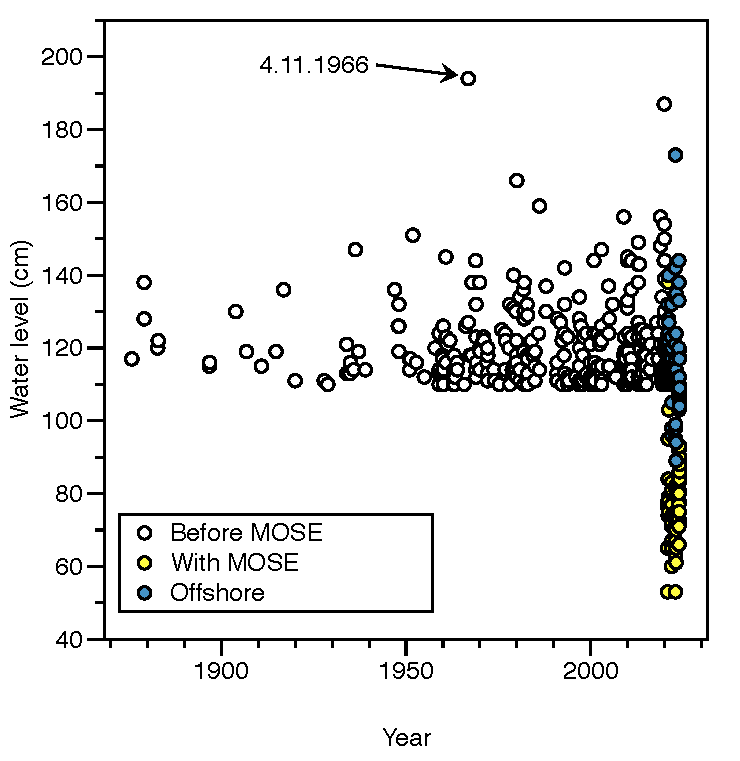
\includegraphics[width=0.9\linewidth]{MOSE effect.pdf}
    \caption{Esempio di grafico che presenta i dati relativi agli eventi di acqua alta nella città di Venezia. La didascalia originale recita: \\ \textit{Acqua Alta in Venice since 1872, as recorded by official sources. The white dots show the data inside the Lagoon before MOSE while the yellow dots after the MOSE was first operated in 2023. The blue dots show the same events as the yellow dots, but measured offshore. The arrow shows the magnitude of the event on November 4\textsuperscript{th}, 1966. Data from Cittá di Venezia (CC-BY 4.0 - https://creativecommons.org/licenses/by/4.0)}}
    \label{fig:graph_example}
\end{figure}

Mentre le figure possono essere estremamente utili per rappresentare un grande volume di dati complessi, che sarebbe difficile o addirittura impossibile riportare in maniera efficace in una tabella, le tabelle, d’altra parte, possono risultare molto pratiche quando si tratta di presentare una serie più limitata di dati, o in situazioni in cui è essenziale fornire al lettore valori numerici precisi. Questo perché le tabelle permettono di evitare di scrivere lunghi blocchi di testo che, in molti casi, potrebbero risultare convoluti o difficili da seguire. Inoltre, quando si utilizzano le tabelle, si può evitare di ripetere numerose informazioni che altrimenti andrebbero presentate in forma discorsiva, cosa che non solo allunga inutilmente il testo, ma rischia di confondere il lettore, che potrebbe perdere il filo logico del discorso. Ad esempio, se dovessimo elencare tutte le maggiori acque alte registrate a Venezia nel corso degli anni, potremmo farlo in un lungo testo scritto, come il seguente:

\textit{“Nel corso della storia recente, le maggiori acque alte registrate a Venezia sono state molte. Ad esempio, il 4 novembre 1966 si è raggiunto un livello di +194 cm, mentre il 12 novembre 2019 il livello dell’acqua ha toccato i +187 cm. In un altro caso, il 22 dicembre 1979, il livello ha raggiunto i +166 cm. Andando avanti, l’1º febbraio 1986, il livello dell’acqua ha toccato +158 cm. Successivamente, il 1º dicembre 2008, si è verificato un altro evento significativo con un livello di +156 cm, seguito da un evento simile il 29 ottobre 2018, quando l’acqua ha raggiunto nuovamente +156 cm. Anche il 15 novembre 2019 si è raggiunto un livello elevato di +154 cm. Nel passato, un altro esempio di alta marea significativa è avvenuto il 12 novembre 1951, con un livello di +151 cm. Successivamente, il 17 novembre 2018 si è registrato un livello di +150 cm, e infine, l’11 novembre 2012, si è toccato un livello di +149 cm.”}

Come si può vedere, un testo di questo tipo non solo risulta particolarmente lungo, ma diventa anche ripetitivo e difficile da seguire. In alternativa, tutti questi dati possono essere riportati in modo molto più chiaro e conciso utilizzando una tabella, come mostrato nella \autoref{tab:acque_alte}, che consente al lettore di visualizzare immediatamente i valori e le date corrispondenti senza dover leggere un lungo paragrafo discorsivo.

\begin{table}[h!]
\centering
\begin{tabular}{cc}
\hline
\textbf{Livello raggiunto (cm)} & \textbf{Data} \\ \hline
+194 & 4 novembre 1966 \\ 
+187 & 12 novembre 2019 \\
+166 & 22 dicembre 1979 \\
+158 & 1º febbraio 1986 \\
+156 & 1º dicembre 2008 \\
+156 & 29 ottobre 2018 \\
+154 & 15 novembre 2019 \\
+151 & 12 novembre 1951 \\
+150 & 17 novembre 2018 \\
+149 & 11 novembre 2012 \\ \hline
\end{tabular}
\caption{Maggiori acque alte registrate a Venezia. Data from Cittá di Venezia (CC-BY 4.0 - https://creativecommons.org/licenses/by/4.0)}
\label{tab:acque_alte}
\end{table}

Nel testo principale di un documento tecnico-scientifico si evitano spesso figure ridondanti o tabelle troppo lunghe. Questi elementi possono essere inseriti nei "Supplementary materials", descritti in seguito.

\subsection{Discussioni}
La sezione delle \textbf{Discussioni} è il momento in cui i risultati ottenuti vengono interpretati e contestualizzati rispetto alla letteratura esistente e agli obiettivi dello studio. In questa sezione, l’autore deve spiegare il significato dei risultati, discutere se questi confermano o contraddicono le ipotesi di partenza, e analizzare eventuali discrepanze o limitazioni emerse durante lo studio.

È importante che le discussioni siano strutturate in modo logico, partendo dai risultati più importanti per poi collegarli ai temi più ampi trattati nella letteratura di riferimento. In questa sezione, occorre evitare di ripetere semplicemente i dati presentati nella sezione dei risultati; piuttosto, occorre che chi scrive concentri la propria attenzione sulle implicazioni di tali dati.

Le discussioni dovrebbero rispondere alle seguenti domande chiave:
\begin{itemize}
	\item Cosa significano i risultati? Spiegare perché i risultati sono importanti e come contribuiscono alla comprensione del problema di ricerca.
	\item Come si confrontano con la letteratura esistente? Discutere se i risultati sono coerenti con studi precedenti o se offrono nuove prospettive o contraddizioni.
	\item Quali sono i limiti dello studio? Riconoscere eventuali limitazioni metodologiche o incertezze nei risultati e spiegare come potrebbero influenzare le conclusioni.
	\item Quali sono le implicazioni future? Suggerire eventuali direzioni per ricerche future, basate su ciò che i risultati hanno rivelato.
\end{itemize}

Un’attenzione particolare deve essere posta nell’evitare di sovra interpretare i risultati, tirando conclusioni che non sono supportate dai dati. Le discussioni devono rimanere ancorate ai risultati ottenuti, fornendo una valutazione obiettiva e critica dello studio, e suggerendo possibili applicazioni pratiche o sviluppi futuri.

Dalla descrizione precedente, appare chiaro che questa sezione deve necessariamente includere citazioni a studi precedenti, in modo da contestualizzare i risultati e confrontarli con la letteratura esistente. Inoltre, può essere utile inserire figure che visualizzino il confronto tra i risultati dello studio e quelli ottenuti in ricerche precedenti, evidenziando somiglianze, differenze o tendenze emergenti. Questa sezione svolge un ruolo chiave nella costruzione dell’argomentazione scientifica, gettando le basi per la sezione conclusiva, dove verranno sintetizzati i risultati principali e delineate le implicazioni future dello studio.

\subsection{Conclusioni}
La sezione delle \textbf{Conclusioni} rappresenta il momento di sintesi e riflessione sui principali risultati emersi dallo studio. Qui si devono riassumere brevemente i risultati chiave, mettendo in evidenza come questi rispondano agli obiettivi iniziali o alle domande di ricerca. È importante che le conclusioni siano concise e mirate, senza ripetere dettagli già discussi in precedenza.

Un buon punto di partenza per le conclusioni è rispondere chiaramente alla domanda: \textit{Quali sono i principali contributi di questo studio?} In questa fase, è utile sottolineare gli aspetti innovativi o le scoperte più rilevanti e, se applicabile, evidenziare come i risultati possono essere utili in un contesto pratico o per sviluppi futuri della ricerca.

È altrettanto importante riconoscere le limitazioni dello studio, spiegando come queste potrebbero aver influenzato i risultati e suggerendo possibili miglioramenti o approcci alternativi per ricerche future.

Infine, nelle conclusioni è utile fare un accenno alle prospettive future: quali sono le direzioni che la ricerca potrebbe prendere a partire dai risultati ottenuti? Quali altri aspetti meriterebbero un approfondimento? Questa parte deve essere visionaria, ma realistica, mostrando come il lavoro presentato si inserisca all’interno di un più ampio panorama scientifico o pratico.

In generale, la sezione conclusiva è più breve rispetto alle altre parti del manoscritto. Sebbene possa includere alcune citazioni chiave, queste devono essere limitate a quelle più rilevanti per ribadire punti fondamentali o collegare i risultati alle implicazioni più ampie della ricerca. Solitamente, le conclusioni non contengono figure o tabelle, poiché il focus è sulla sintesi e non sulla presentazione di nuovi dati o approfondimenti visivi. È importante ricordare che, di solito, non si conclude un lavoro scientifico con una citazione di altri autori.

\subsection{Ringraziamenti}
La sezione dei \textbf{Ringraziamenti} è il luogo dove gli autori possono riconoscere il supporto ricevuto durante il corso della ricerca. È opportuno ringraziare persone, agenzie di finanziamento, enti esterni all’istituzione di appartenenza che hanno fornito assistenza, strumentazione o dati. Questo può includere anche enti o organizzazioni che hanno condiviso dati, citando le fonti come richiesto dai terms of service. È importante mantenere la sezione concisa ed evitare frasi prolisse o personali, concentrandosi sugli aspetti professionali e tecnici del supporto ricevuto.

\begin{info}
\textbf{Esempio di cosa NON scrivere:}
\textit{“Vorrei ringraziare mia madre e mio padre per il loro continuo supporto morale e mio fratello per avermi aiutato con la revisione del testo. Un grazie speciale va ai miei amici, che mi hanno dato l’ispirazione durante i momenti difficili.”}

Questo esempio include elementi troppo personali e non pertinenti per un documento tecnico-scientifico.

\textbf{Esempio di cosa scrivere:}
\textit{“Gli autori desiderano ringraziare l’agenzia XYZ per il finanziamento di questo progetto (grant n. 12345), e l’ente ABC per aver fornito i dati meteorologici utilizzati nell’analisi. Si ringraziano inoltre il Dr. Mario Rossi per il supporto tecnico e la consulenza statistica, e il laboratorio DEF per aver messo a disposizione le attrezzature necessarie allo svolgimento degli esperimenti.”}

Questo esempio è conciso, professionale e si concentra esclusivamente sui contributi rilevanti alla ricerca, evitando toni personali o prolissi
\end{info}

È comprensibile che, specialmente in una tesi, studentesse e studenti vogliano esprimere ringraziamenti personali a genitori, amici o altre persone che li hanno supportati emotivamente durante il percorso di studi. Tuttavia, questi tipi di ringraziamenti personali non sono appropriati nella sezione dei ringraziamenti di un documento tecnico-scientifico. Se si desidera includerli, è consigliabile inserirli in una \textbf{prefazione}, che è lo spazio più adatto per esprimere gratitudine personale e riflessioni personali legate al proprio percorso.

\subsection{Bibliografia}    
La \textbf{bibliografia} è una componente fondamentale di qualsiasi documento tecnico-scientifico, in quanto permette di dare credito alle fonti utilizzate e di offrire al lettore la possibilità di approfondire gli argomenti trattati. Di seguito sono riportate le regole essenziali per stilare correttamente la bibliografia e per citare le fonti nel testo.

\begin{enumerate}
	\item Le voci bibliografiche devono essere elencate in ordine alfabetico per autore, o in ordine numerico a seconda del sistema di citazione adottato.
	\item Ogni voce deve includere tutte le informazioni necessarie per identificare la fonte. In genere, ciò comprende:
    \begin{itemize}
	\item Nome e cognome degli autori
	\item Titolo dell’articolo, del libro o del capitolo
	\item Nome della rivista o dell’editore
	\item Volume, numero, pagine (se applicabile)
	\item Anno di pubblicazione
	\item DOI o URL (per le fonti online, se rilevante)
     \end{itemize}
	\item Lo stile di citazione deve essere uniforme. Esistono diversi stili di citazione (ad es. APA, MLA, Chicago, IEEE), quindi è importante scegliere uno stile appropriato e applicarlo in modo coerente in tutto il documento.
	\item Libri, articoli di rivista, capitoli di libri e fonti online seguono formati bibliografici leggermente diversi. Assicurati di rispettare le differenze di formato tra le diverse tipologie di fonti.
\end{enumerate}

Ogni lavoro citato nel testo deve essere presente nella bibliografia finale, e ogni fonte elencata in bibliografia deve essere citata nel corpo del testo. Ciò garantisce coerenza e trasparenza, facilitando al lettore la verifica e l’approfondimento delle informazioni presentate. Inoltre, è importante evitare di citare fonti generiche o difficilmente reperibili: ogni citazione deve fornire informazioni complete e accessibili.

Le citazioni devono essere puntuali e pertinenti, evitando di accumulare riferimenti non necessari. Ogni volta che si introduce un concetto derivato da una fonte esterna, la citazione deve essere inserita immediatamente dopo l’informazione riportata, in modo che il lettore sappia esattamente da dove proviene l’idea. Le citazioni possono riguardare sia studi classici e consolidati, sia ricerche recenti che arricchiscono la discussione o ne estendono i confini.

Ecco alcune regole da tenere a mente quando vengono scelte le citazioni:

\begin{enumerate}
	\item Le fonti devono essere citate nel testo in accordo con lo stile bibliografico scelto. Per esempio, nello stile APA, si cita con il formato “(Autore, anno)” nel corpo del testo, mentre in IEEE si usano numeri tra parentesi quadre [1].
	\item Ogni volta che si fa riferimento a un’idea, un dato o un risultato proveniente da una fonte esterna, questa deve essere citata. È importante non limitarsi a citare fonti solo alla fine del paragrafo, ma farlo puntualmente dopo ogni affermazione rilevante.
	\item Se una stessa affermazione si basa su più fonti, queste possono essere elencate all’interno della stessa citazione (ad es. “(Autore1, anno; Autore2, anno)”).
	\item Anche le fonti online devono essere citate correttamente. È necessario includere non solo l’URL, ma anche la data di accesso, in quanto le pagine web possono essere modificate nel tempo.
\end{enumerate}

Ecco un esempio di testo con relative citazioni (ATTENZIONE! Le citazioni in questo testo sono inventate!)

\begin{info}
L’erosione costiera rappresenta un problema crescente per molte aree urbane costiere, particolarmente in relazione all’aumento della frequenza delle mareggiate violente. Secondo Rossi (2020), l’intensificazione di questi eventi climatici estremi è una delle principali cause del fenomeno, con conseguenze sempre più gravi per l’integrità delle spiagge. Tuttavia, le strutture di protezione costiera, come le barriere frangiflutti, spesso non forniscono una protezione sufficiente, soprattutto in condizioni di mareggiate straordinarie (Bianchi e Verdi, 2018). Inoltre, l’innalzamento del livello del mare, dovuto ai cambiamenti climatici, sta ulteriormente aggravando la situazione, rendendo le città costiere sempre più vulnerabili (Ferrari et al. 2021).

\textbf{Bibliografia}

Bianchi, G., Verdi, F. (2018). Barriere costiere: Una soluzione inadeguata? Studi di Protezione Ambientale, 12(1), 78-89.
 
Ferrari, M., Russo, L., Neri, S. (2021). L’innalzamento del livello del mare e l’impatto sulle città costiere. Journal of Environmental Studies, 33(4), 145-160.

 Rossi, L. (2020). Erosione costiera e mareggiate: Un’analisi recente. Rivista di Geografia Costiera, 45(3), 234-256.
\end{info}

In un documento tecnico-scientifico, la grande maggioranza delle citazioni sono riferite ad articolo cosiddetti \textit{peer-reviewed}, ovvero contributi pubblicati su riviste scientifiche dopo un processo di revisione da parte di esperti del settore, e dopo un attento controllo editoriale della veridicità e solidità scientifica dei risultati. Un buon motore di ricerca per articoli \textit{peer reviewed} è \href{https://scholar.google.com}{Google Scholar}, che indicizza i lavori scientifici (e in parte documenti tecnici) da molte fonti, inviando l'utente al PDF dell'articolo (se disponibile liberamente) o alla pagina della rivista (da cui si può accedere all'articolo se la libreria della propria istituzione ha un abbonamento alla rivista o alla casa editrice).

A volte, soprattutto per quanto riguarda le fonti di dati, possono essere citati rapporti tecnici o siti istutuzionali, che comunque hanno una garanzia di longevità e spesso hanno controlli editoriali interni, anche se non sono \textit{peer reviewed}. Sono generalmente da evitare citazioni a dispense online, siti generalisti o altre fonti online, ad esempio Wikipedia. Se si trova un'affermazione particolarmente importante su una di queste fonti, occorre indagare la fonte primaria e riportare quella (Wikipedia cita molto spesso articoli scientifici a supporto dei suoi contenuti). 

\subsection{Supplementary materials}
I \textbf{Supplementary Materials} sono utilizzati per fornire dati e informazioni aggiuntive che completano l’articolo principale, ma che per motivi di spazio o dettaglio non possono essere inseriti nel corpo del testo. Questi materiali possono includere dataset completi, codici utilizzati per le analisi, grafici supplementari, tabelle di dati dettagliate, metodologie estese o descrizioni di esperimenti aggiuntivi. È importante che le informazioni contenute nei Supplementary Materials siano direttamente rilevanti per la comprensione e la riproducibilità dello studio, e che vengano organizzate in modo chiaro e accessibile per i lettori interessati ad approfondire i dettagli tecnici o metodologici.

\section{Stesura del testo}
Per quanto riguarda lo stile di scrittura, un documento tecnico-scientifico deve essere caratterizzato da chiarezza, precisione e semplicità. Le frasi dovrebbero essere brevi e dirette, in modo da facilitare la comprensione e ridurre la possibilità di fraintendimenti. È importante evitare l’uso eccessivo di avversative all’interno della stessa frase, poiché ciò può confondere il lettore o rendere il discorso meno fluido. Frasi troppo lunghe e complesse dovrebbero essere evitate, in quanto tendono a sovraccaricare l’attenzione del lettore e possono far perdere il filo logico dell’argomentazione. Un buon principio è quello di esprimere un solo concetto principale per frase, mantenendo il testo conciso e lineare. L’obiettivo è rendere il documento accessibile a un pubblico scientifico che desidera assimilare rapidamente le informazioni, senza compromettere la precisione tecnica.

In generale, è utile suddividere il testo in paragrafi, separati tra loro da un capoverso o da uno spazio (come in questo testo). Ogni paragrafo dovrebbe essere composto da 4-5 frasi e avere l’obiettivo di fornire un’informazione chiara al lettore, che risulti utile per comprendere o contestualizzare il paragrafo successivo.

\subsection{Plagio nei testi}
Un documento tecnico-scientifico deve essere un’opera originale, frutto del lavoro intellettuale e della scrittura degli autori. È quindi fondamentale evitare ogni forma di plagio, che è una violazione dell’integrità accademica e scientifica. Il plagio è definito e regolato all’interno di molti regolamenti accademici e linee guida di riviste scientifiche. Ad esempio, le linee guida per la stesura delle tesi dell’ \textcite{plagio} definiscono il plagio come: \textit{“la parziale o totale attribuzione di parole, idee, ricerche o scoperte altrui a se stessi o nell’omissione della citazione delle fonti.”}

Il plagio può assumere diverse forme, dall’uso non autorizzato di testi, idee o risultati, all’omissione delle citazioni appropriate. Questo include non solo il copia-incolla di parti di testi senza riconoscere la fonte, ma anche la parafrasi di idee altrui senza adeguata attribuzione.

Oltre ad essere esplicitamente vietato dai regolamenti accademici, il plagio è considerato un illecito anche sul piano legale. La legge n. 475/1925, modificata nel 1999, stabilisce che presentare come propri lavori, in tutto o in parte copiati, costituisce un reato punibile con la reclusione da tre mesi ad un anno (nel caso in cui il plagio avvenga su documenti ufficiali, quali una tesi di laurea o di dottorato). È quindi essenziale attribuire correttamente ogni fonte utilizzata, sia nel testo che nella bibliografia, per garantire la correttezza scientifica e il rispetto delle norme legali.

Ecco una serie di regole che occorre tenere a mente per evitare qualsiasi forma di plagio durante la scrittura:
\begin{enumerate}
\item \textbf{Copiare testi senza citare la fonte}: copiare interi passaggi o estratti da articoli, libri o siti web senza menzionare la fonte costituisce plagio. Anche quando il testo sembra descrivere fatti noti, è sempre necessario attribuire correttamente l’origine delle parole e delle idee. Ogni volta che viene utilizzato anche un piccolo estratto di testo, è necessario renderlo con parole proprie e includere una citazione corretta.

\item \textbf{Parafrasare senza citare}: anche quando un testo viene parafrasato, è comunque necessario dare credito all’autore originale. Parafrasare non trasferisce la proprietà intellettuale delle idee, e i concetti o le teorie provenienti da fonti esterne devono sempre essere attribuiti all’autore originale.

\item \textbf{Utilizzare immagini, grafici o tabelle senza attribuzione}: oltre al testo scritto, anche i materiali visivi, come immagini, grafici e tabelle, devono essere correttamente attribuiti. Non basta inserirli nel documento; è necessario indicare chiaramente la fonte da cui provengono, anche se modificati o adattati per il lavoro.

\item \textbf{Riutilizzare lavori precedenti (auto-plagio)}: l’auto-plagio si verifica quando un lavoro precedentemente creato o pubblicato viene presentato come nuovo senza indicarlo. Anche se si è l’autore originale, riutilizzare testi, dati o idee senza menzionare la pubblicazione precedente costituisce una violazione dell’integrità accademica. Per evitarlo, è sempre opportuno citare il proprio lavoro passato.

\item \textbf{Non citare correttamente le fonti}: menzionare una fonte non è sufficiente; è importante citare correttamente ogni riferimento secondo lo stile bibliografico richiesto (es. APA, MLA, IEEE). Citazioni errate, incomplete o mal formattate possono essere considerate plagio non intenzionale, ma comunque scorretto. È quindi necessario seguire attentamente il formato di citazione appropriato per ogni fonte utilizzata.

\item \textbf{Sottovalutare la necessità di citare dati pubblici o comuni}: anche se una fonte riporta dati pubblici (come statistiche governative o fatti noti), è comunque necessario citare la fonte specifica da cui tali dati provengono. Il fatto che un’informazione sia accessibile pubblicamente non esime dall’obbligo di attribuzione, poiché la chiarezza delle fonti conferisce credibilità al lavoro.

\item \textbf{Omettere di citare contributi secondari}: quando vengono utilizzate idee o analisi derivate da ricerche precedenti, è importante citare anche quei contributi secondari. Ad esempio, se uno studio si basa su una metodologia sviluppata in un altro articolo, tale articolo dovrebbe essere citato, anche se non rappresenta la fonte diretta dei dati. Questo riconosce l’influenza delle opere precedenti nel lavoro svolto.

\item \textbf{Usare software di traduzione o tradurre manualmente un testo senza citare la fonte}: tradurre un testo da una lingua all’altra non rende automaticamente il contenuto originale. Anche se le parole cambiano, l’idea e la struttura rimangono quelle dell’autore originale. È quindi necessario citare sempre la fonte originale del testo tradotto per garantire la corretta attribuzione dell’opera, indipendentemente dal fatto che la traduzione sia manuale o assistita da software.

\item \textbf{Citare verbatim senza virgolette o attribuzione}: quando si riportano esattamente le parole di un altro autore (citazione verbatim), il testo deve essere racchiuso tra virgolette e accompagnato da una citazione corretta, indicante l’autore, l’anno e, se applicabile, il numero di pagina. Omettere virgolette o un’attribuzione corretta costituisce plagio. Anche brevi estratti testuali devono essere citati con precisione per rispettare i diritti dell’autore originale.

\end{enumerate}

Ecco un esempio di come un testo può venire utilizzato, citandone correttamente la fonte.

\begin{info}
Quando si riporta una frase esattamente come appare nella fonte originale, si tratta di una citazione verbatim. In questi casi, è necessario racchiudere il testo tra virgolette e citare correttamente l’autore e la pagina o sezione specifica da cui è stata tratta l’informazione. È importante non modificare il contenuto della citazione e fornire un riferimento accurato.

Esempio di testo originale, scritto da Rossi, 2020, pagina 45 (ATTENZIONE! il riferimento è inventato!)

\textit{“L’erosione costiera è un processo naturale che può essere accelerato da interventi umani, come la costruzione di strutture artificiali lungo le coste.”}

Questo testo può essere citato parafrasando il testo, come in questo esempio:

\textit{Secondo Rossi (2020), l’erosione delle coste è un fenomeno naturale, che può venire intensificato dalle attività umane, ad esempio quando si costruiscono strutture artificiali (ad esempio, porti o isole artificiali).}

Oppure può essere citato parola per parola, ma deve essere evidenziato in questo modo:

\textit{“L’erosione costiera è un processo naturale che può essere accelerato da interventi umani, come la costruzione di strutture artificiali lungo le coste.” (Rossi, 2020, p. 45)}

In questo esempio, la citazione verbatim riporta esattamente le parole dell’autore originale, mentre la parafrasi riscrive il concetto con parole diverse, mantenendo comunque il significato originale e citando correttamente la fonte. In un documento tecnico-scientifico, si può ricorrere alla citazione verbatim solo in casi rari e ben definiti, in cui il concetto da rendere o l'autore siano particolarmente importanti.
\end{info}

Una eccezione che può essere fatta al plagiarismo nei testi è quando si riportano verbatim procedure particolari, come per esempio analisi di laboratorio o i passaggi di una catena di modellizzazione che sono stati adottati da altre fonti. In questo caso potrebbe essere necessario che la descrizione del metodo venga mantenuta identica per evitare incomprensioni ed errori nella riproduzione del lavoro. Tuttavia, anche in questi casi, è necessario evidenziare correttamente come la procedura o l'analisi descritte siano derivate da altre fonti e non il risultato del lavoro degli Autori.

\subsection{Uso di intelligenza artificiale}
L'Intelligenza Artificiale (IA) sta diventando uno strumento sempre più importante, che può fornire una assistenza concreta alla scrittura e all'organizzazione di un documento tecnico-scientifico. Tuttavia, il suo utilizzo sta generando anche dei complessi, e ancora non del tutto risolti, problemi etici. Per esempio, ci si potrebbe porre la domanda: \textit{se un testo ha molte parti generate dall'IA, si può ancora considerare un contributo originale degli autori?} Inoltre, le informazioni generate da una IA senza un controllo rigoroso possono risultare scorrette, incomplete o errate. Spesso non vengono fornite citazioni delle fonti (o, nei casi limite, vengono generate citazioni inesistenti).

L'\textcite{IA}, nelle linee guida dedicate alla stesura di una tesi ed utilizzo di intelligenza artificiale, riporta quanto segue:

\textit{"L'elaborazione della tesi di laurea richiede sia la capacità di generare contenuti originali e argomentazioni ben strutturate, che un'ampia comprensione del campo di studio e delle metodologie di ricerca utilizzate. L’intelligenza artificiale generativa (AI) e le tecnologie da essa assistite, come ChatGPT o servizi simili, possono essere strumenti utili per la stesura della tesi, ma devono essere usati con cautela, consapevolezza dei limiti e trasparenza. Nel caso di utilizzo dell’AI per migliorare il linguaggio e la leggibilità, per organizzare il testo generando outline e schemi che guidino la scrittura o per l'analisi di grandi quantità di dati, è importante che il contributo fornito dall’AI sia riconoscibile e che sia comunque sottoposto a rielaborazione critica e revisione personale. Per evitare il plagio, inoltre, in un elaborato di laurea è essenziale riportare i riferimenti bibliografici e le fonti esterne a cui fa riferimento una sezione di testo, attività spesso difficile in caso di testi generati da AI. Si suggerisce pertanto di porre estrema cautela nell’utilizzo dell’AI e, nel caso sia stata utilizzata nella stesura della tesi di laurea, si chiede di includere una sezione dedicata alla fine dell’elaborato nella quale viene specificato in che modo e in che parti della tesi è stata utilizzata l’AI e nella quale ci si assume la piena responsabilità dei contenuti."}

In sostanza, l’IA può facilitare il lavoro degli autori suggerendo frasi o strutture più fluide, ma non deve sostituire il pensiero critico e l’analisi rigorosa che sono alla base della scrittura scientifica. Occorre inoltre essere trasparenti su come sia stata utilizzata l'IA in un documento tecnico scientifico.

In questo documento, è stato utilizzato ChatGPT in alcune sezioni per migliorare la struttura di alcuni concetti e rendere più scorrevoli alcuni paragrafi. Questo strumento ha permesso di affinare l’organizzazione delle idee, mantenendo la coerenza e la fluidità del testo. Tuttavia, è stato essenziale mantenere un controllo critico sui suggerimenti forniti, valutandone l’adeguatezza rispetto al contenuto originale.

\begin{info}    
Ad esempio, per il primo paragrafo, la versione iniziale era la seguente:

\textit{"La scrittura tecnico-scientifica è una delle competenze più richieste nel mercato del lavoro per chi opera nel campo delle scienze ambientali. In ambito professionale, infatti, non è raro di dover scrivere rapporti tecnici per aziende, enti, e altri tipi di committenti. Solitamente, il rapporto tecnico in seguito a una consulenza, un'opera o una serie di analisi è il documento che segna l'avanzamento o la conclusione dei lavori, al quale spesso corrisponde l'emissione di una fattura da parte del consulente verso il committente. In modo analogo, a livello universitario, la tesi (di laurea o di dottorato) è un documento tecnico-scientifico (con valore legale) che suggella la fine del percorso accademico di una studentessa o uno studente."}

È stato poi chiesto a ChatGPT di migliorare questo paragrafo, utilizzando il seguente prompt:
\textit{"Sto scrivendo un testo per insegnare le regole di base per la scrittura tecnico-scientifica a studentesse e studenti universitari. Aiutami a migliorare i miei paragrafi."}

A partire da questo input, ChatGPT ha suggerito delle modifiche che hanno reso il paragrafo più fluido e preciso, mantenendo comunque il senso originale. Ecco la versione rielaborata:

Versione migliorata da ChatGPT: \textit{"La scrittura tecnico-scientifica è una delle competenze più richieste nel mercato del lavoro per i professionisti del settore ambientale. Nel contesto professionale, infatti, è comune dover redigere rapporti tecnici per aziende, enti o altri committenti. Tali rapporti, redatti a seguito di consulenze, opere o analisi, spesso rappresentano l’avanzamento o la conclusione di un progetto, e sono strettamente legati all’emissione di una fattura da parte del consulente verso il committente. Allo stesso modo, in ambito accademico, la tesi (sia di laurea che di dottorato) è un documento tecnico-scientifico che, con valore legale, segna la conclusione del percorso di studi di una studentessa o uno studente."}

In questo caso, ChatGPT ha riformulato le frasi in modo più scorrevole e ha sostituito alcune espressioni per renderle più concise. Questi miglioramenti sono stati utili per rendere il testo più chiaro, senza alterare il contenuto originale o l'intento comunicativo.
\end{info}

\subsection{Software di scrittura}
Per quanto la scrittura, ci sono vari strumenti che possono essere utilizzati per la stesura di un documento tecnico-scientifico. Tra questi, quelli maggiormente utilizzati sono i software di videoscrittura come Microsoft Word e i suoi equivalenti \textit{open access}, e sistemi di composizione tipografica come LaTeX.

\textbf{Microsoft Word} è uno degli strumenti più diffusi per la scrittura di documenti grazie alla sua interfaccia intuitiva e alla vasta gamma di funzionalità integrate, come il controllo ortografico, la formattazione automatica e i modelli predefiniti. Permette di creare documenti professionali in modo rapido e semplice, e dispone di strumenti per la revisione e la collaborazione, come il track changes e i commenti, utili quando si lavora in gruppo.

Esistono anche alternative \textit{open access}, come \textbf{LibreOffice Writer} e \textbf{Google Docs}, che offrono funzionalità simili a Word, ma con il vantaggio di essere gratuite. LibreOffice Writer supporta la maggior parte dei formati di file e offre molte delle stesse funzionalità di formattazione e revisione. Google Docs, invece, permette una collaborazione in tempo reale, con la possibilità di condividere documenti e lavorare contemporaneamente su di essi, il che lo rende particolarmente utile per progetti di gruppo.

Questi strumenti di videoscrittura sono ideali per documenti semplici o di media complessità, ma possono risultare limitati per la gestione avanzata di equazioni, riferimenti bibliografici o formattazioni specifiche richieste da riviste scientifiche.

Una delle principali difficoltà nell’utilizzo dei software di videoscrittura come Word o LibreOffice è la gestione automatica delle citazioni e la possibilità di formattarle secondo stili bibliografici diversi. Questo può risultare complesso, soprattutto quando si devono rispettare requisiti editoriali specifici o modificare lo stile delle citazioni durante la revisione del documento. Per risolvere questo problema, è possibile utilizzare un software \textit{open access} come \href{https://www.zotero.org}{Zotero}, che consente di creare un database bibliografico organizzato.

Zotero permette di raccogliere, gestire e inserire citazioni di articoli, libri e altre fonti direttamente nel documento. Attraverso l’installazione di un plugin compatibile con Word o LibreOffice, gli autori possono facilmente inserire citazioni nel testo e generare automaticamente la bibliografia. Zotero supporta numerosi stili di citazione, come APA, MLA, Chicago, IEEE e molti altri, permettendo di modificare il formato delle citazioni in modo rapido e senza errori.

È importante notare, tuttavia, che Zotero non può essere utilizzato direttamente con Google Docs, limitando quindi la sua integrazione con strumenti di scrittura collaborativi online.

Un altro software (open source) ampiamente utilizzato nella comunità accademica è \textbf{LaTeX}, uno strumento di composizione tipografica basato su markup. LaTex è utile per redigere documenti che richiedono una formattazione complessa, come tesi, articoli scientifici e documenti che includono numerose equazioni matematiche, figure e riferimenti bibliografici. LaTeX si distingue per la sua capacità di generare documenti di altissima qualità tipografica e per la gestione avanzata di riferimenti incrociati, bibliografie e figure.

A differenza dei software di videoscrittura come Word, LaTeX richiede una conoscenza di base del linguaggio di markup, ma una volta acquisita, permette di creare documenti complessi con un controllo totale sulla formattazione. LaTeX è particolarmente indicato per lavori scientifici, in quanto facilita la gestione di formule matematiche, citazioni, riferimenti bibliografici e tabelle, con un output di altissima qualità.

Esistono editor online come Overleaf, che combinano i vantaggi di LaTeX con un’interfaccia web collaborativa, permettendo di lavorare su documenti in tempo reale e facilitando la collaborazione tra più autori. 

Ad esempio, questo testo è stato scritto con LaTeX proprio in Overleaf.

\section{Figure e tabelle}
Le figure e le tabelle sono componenti essenziali di un documento tecnico-scientifico, poiché permettono di presentare informazioni complesse in modo chiaro e visivamente accessibile. Le tabelle, come già discusso, sono utili per organizzare dati o informazioni che risulterebbero troppo complicate o prolisse se riportate nel testo. Le figure, invece, possono includere grafici, mappe, schemi o altri elementi visivi che aiutano il lettore a comprendere e visualizzare concetti descritti nel testo.

Ci sono tre regole fondamentali per la connessione tra figure/tabelle e il testo scritto. La prima è che ogni figura o tabella deve essere numerata e citata esplicitamente nel testo, in modo che il lettore sappia esattamente a quale elemento visivo si fa riferimento. La seconda è che ogni figura o tabella deve avere una didascalia chiara e concisa che descriva cosa viene rappresentato. Le didascalie sono generalmente collocate sotto le figure e, a volte, sopra le tabelle, in conformità con le linee guida specifiche. Posizionare la didascalia sopra una tabella, in particolare, facilita la comprensione immediata dei dati riportati.  La terza regola è che, per ogni quantità riportata in una tabella o figura, devono essere chiaramente indicate le unità di misura. Questo è essenziale per garantire l’accuratezza e la comprensibilità dei dati presentati, evitando possibili ambiguità. Si vedano come esempio la \autoref{tab:acque_alte} e la \autoref{fig:graph_example} in questo documento. Si noti che l'esempio riportato in \autoref{fig:excel_bad} non ha una etichetta che indichi cosa rappresentano i due assi: \textbf{questo é assolutamente da evitare}.

Una delle sfide maggiori nella realizzazione delle figure in un documento tecnico-scientifico è creare una veste grafica che sia al contempo rigorosa, informativa e visivamente accattivante. Le figure devono essere progettate in modo da comunicare chiaramente i dati, mantenendo un alto livello di precisione scientifica, ma senza trascurare l’aspetto estetico. Una buona figura dovrebbe essere facile da interpretare a colpo d’occhio, con etichette ben leggibili, una scelta cromatica appropriata e un’organizzazione logica degli elementi. È importante evitare grafici sovraccarichi o troppo complessi che potrebbero confondere il lettore, preferendo invece un design pulito e ordinato. L’uso di strumenti di grafica avanzata, come software di elaborazione dati e grafici, può aiutare a ottenere un equilibrio tra accuratezza e presentazione visiva, garantendo che le figure non solo rappresentino correttamente i dati, ma siano anche visivamente accattivanti e professionali. 

Ci sono molti programmi di grafica che possono aiutare a migliorare l'output di una figura. Per esempio, la \autoref{fig:graph_example} è stata realizzata con un software per Mac chiamato "Datagraph", che consente un buon controllo della veste grafica di un elaborato. Tuttavia, si può migliorare di molto la veste grafica di un prodotto anche usando gli strumenti forniti da applicazioni come Microsoft Excel, che non nasce come programma di grafica ma come foglio di calcolo. Per esempio, vediamo come i dati in \autoref{tab:acque_alte} sono riprodotti usando i settaggi di default di Microsoft Excel (\autoref{fig:excel_bad}).

\begin{figure}[h!]
    \centering
    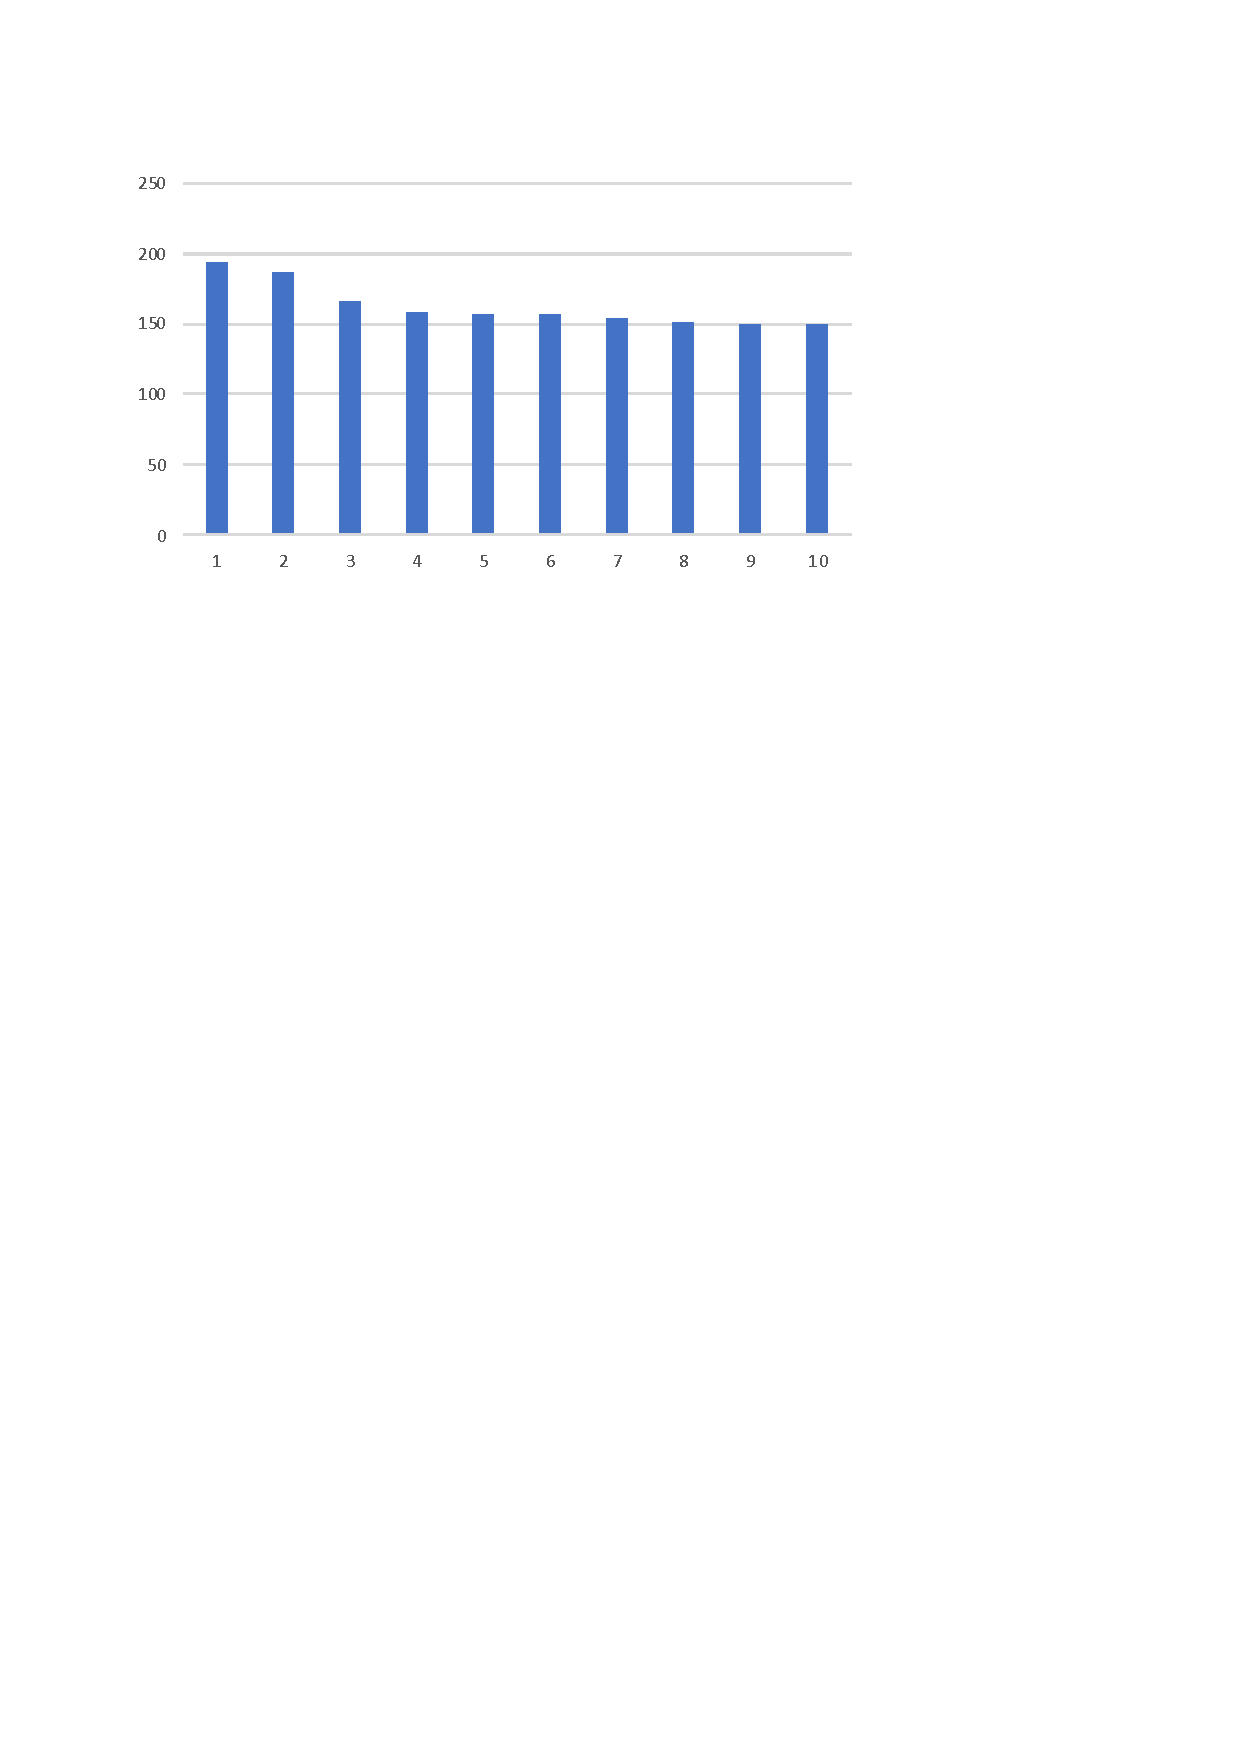
\includegraphics[width=0.9\linewidth]{figures/graph_original.pdf}
    \caption{Esempio di grafico realizzato con MS Excel utilizzando i dati riportati in \autoref{tab:acque_alte}, utilizzando i settaggi di default del programma. Data from Cittá di Venezia (CC-BY 4.0 - https://creativecommons.org/licenses/by/4.0)}
    \label{fig:excel_bad}
\end{figure}

Con un po' di lavoro sul layout di MS Excel, il risultato grafico può migliorare di molto, come evidenziato in \autoref{fig:excel_good}. Ecco quali sono stati i cambiamenti che sono stati fatti al layout originale presentato in \autoref{fig:excel_bad}:

\begin{itemize}
    \item Inserito etichette sugli assi X e Y per comunicare al lettore cosa rappresenta il grafico.
    \item Corretto l'asse X di modo che le etichette rappresentassero le date e non i numeri di riga.
    \item Cambiato lo spessore di asse X e asse Y, e cambiato colore in nero
    \item Il font delle etichette degli assi è stato aumentato da 9 a 12 punti. 
    \item è stato inserito il titolo sull'asse delle ordinate (asse Y).
    \item è stata eliminata la griglia, sono state inseriti i tick marks sull'asse delle ordinate ed è stato aggiunto il bordo su tutta l'area del grafico.
    \item Per ridurre lo spazio bianco, il massimo sull'asse delle ordinate è stato ridotto a 200.
    \item è stata aumentata la dimensione delle barre e ne è stato cambiato il colore, e le etichette sull'asse delle ascisse sono state inserite all'interno del grafico e il font è stato cambiato da regular a bold (grassetto), con colore bianco.
\end{itemize}

\begin{figure}[h!]
    \centering
    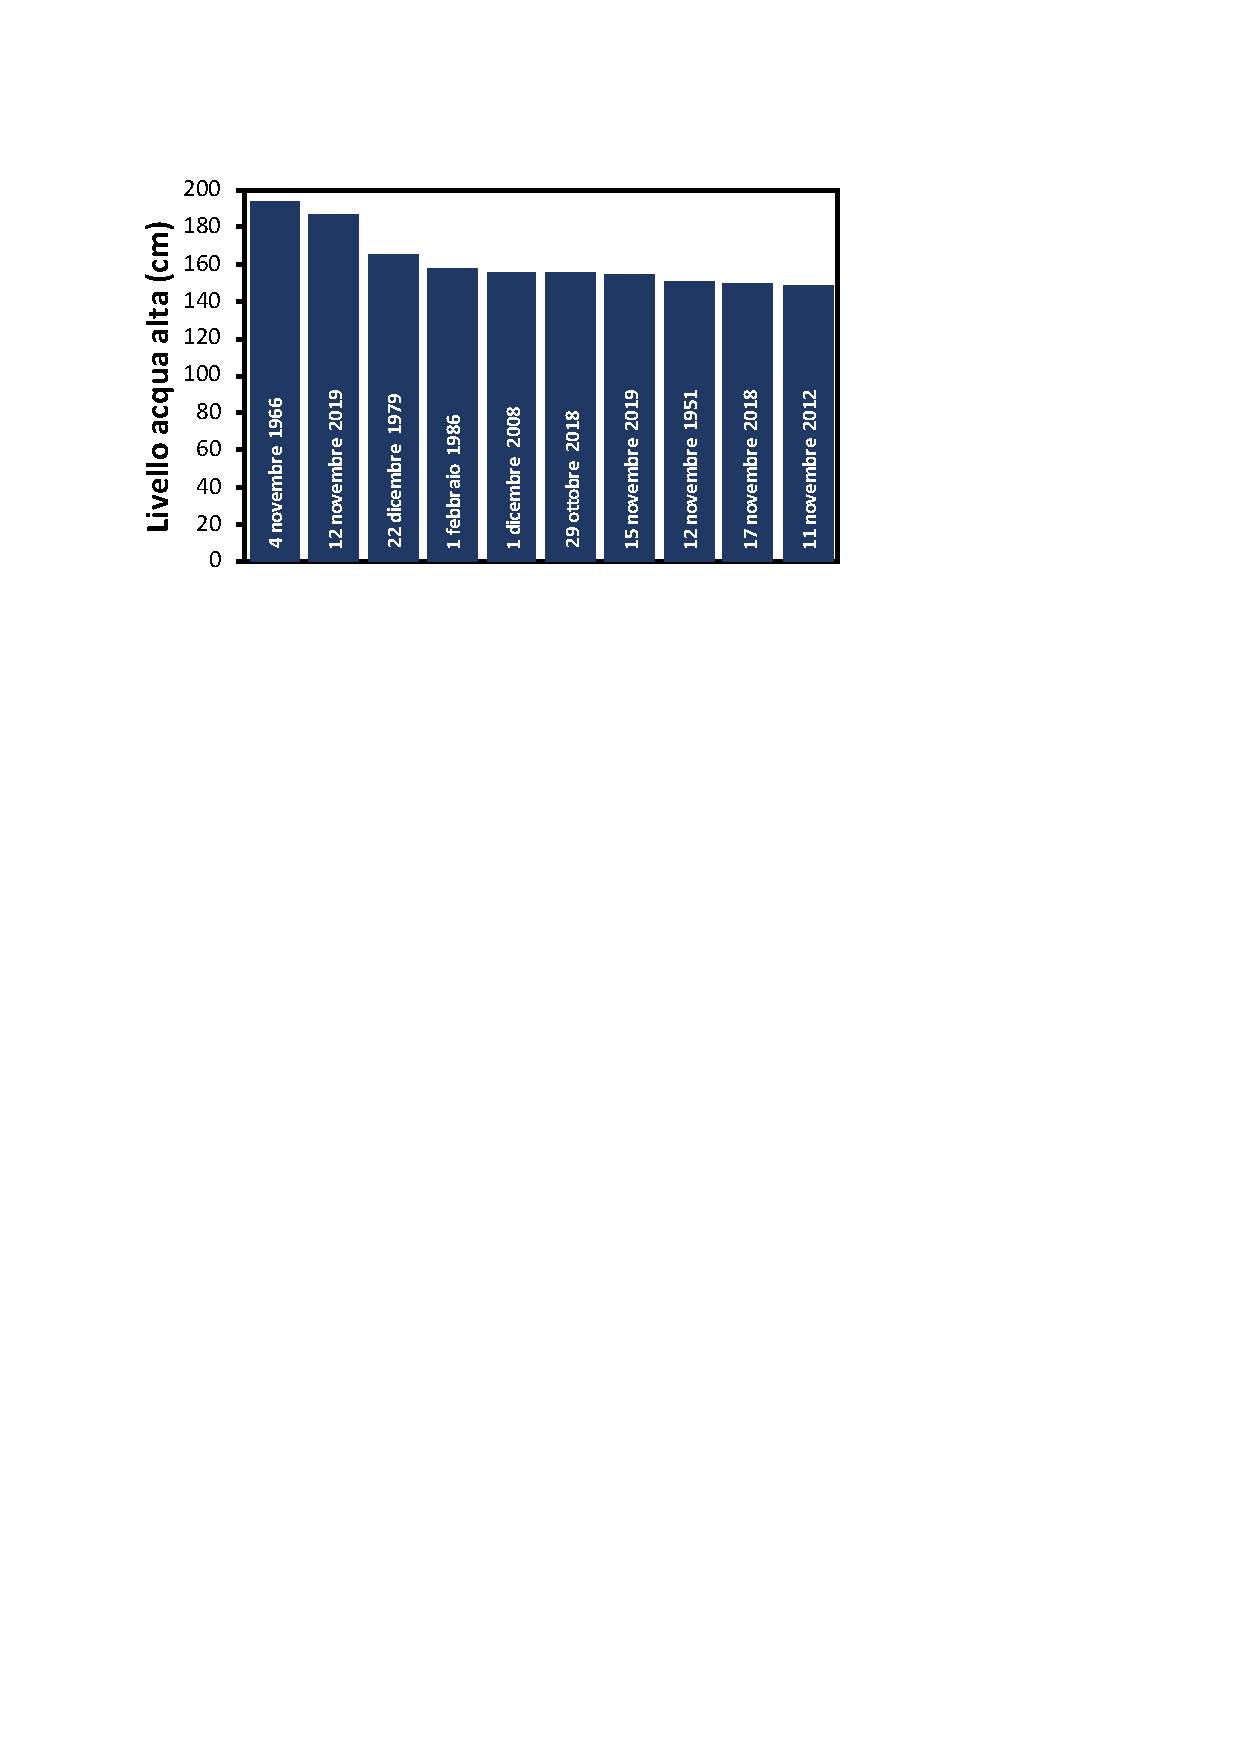
\includegraphics[width=0.9\linewidth]{figures/graph_custom.pdf}
    \caption{Esempio di grafico realizzato con MS Excel utilizzando i dati riportati in \autoref{tab:acque_alte}, modificando le proprietà del grafico tramite gli strumenti forniti dal software. Data from Città di Venezia (CC-BY 4.0 - https://creativecommons.org/licenses/by/4.0)}
    \label{fig:excel_good}
\end{figure}

Rispetto alla \autoref{fig:excel_bad}, la \autoref{fig:excel_good} usa meglio lo spazio a disposizione, fornisce informazioni dettagliate sui dati rappresentati (es. date delle acque alte storiche più elevate) e ha una dimensione dei caratteri leggibile e adeguata alla dimensione dei caratteri del testo principale.

Spesso, è necessario dividere le figure in \textit{panels}, ovvero in sottofigure diverse che contengono informazioni diverse ma comunque correlate tra loro. Si veda, come esempio, la \autoref{fig:map_example}, dove sono presenti due sottofigure, identificate come a) e b), e descritte separatamente nella legenda. In questo caso, spesso le due figure vengono prodotte separatamente (ma con le stesse caratteristiche di font, colori e stile) e unite tramite programmi di grafica. Un programma di utilizzo comune per questa operazione (e per sovrapporre etichette o altri elementi) è \href{https://inkscape.org}{Inkscape}, che è gratuito e funziona su tutti i sistemi operativi.

Un’ultima cosa da tenere a mente è che le figure devono essere di alta qualità. In questo documento, le figure sono state realizzate in formato PDF, il che significa che sono vettoriali e possono essere ridimensionate senza perdita di risoluzione. Quando si preparano figure per la stampa, è importante considerare la risoluzione, espressa in DPI (dots per inch). Per garantire che le immagini stampate siano nitide e chiare, le figure raster (come JPEG o PNG) dovrebbero essere preparate con una risoluzione di almeno 300 DPI per stampe standard. Se il documento è destinato a una rivista scientifica o a un lavoro di alta qualità, si consiglia di utilizzare una risoluzione di 600 DPI o superiore. In ogni caso, l’obiettivo è ottenere immagini che rimangano chiare e leggibili, sia che vengano visualizzate su schermo o stampate.

\subsection{Riutilizzo di immagini}
Durante la stesura di un elaborato tecnico-scientifico, può capitare di doversi trovare nella situazione di dover riutilizzare immagini (o parti di esse) da altre fonti. Un esempio di come riutilizzare una parte di una immagine è presentata in \autoref{fig:map_example}, dove le immagini di background non sono frutto del lavoro dell'autore, ma sono riprodotte da fonti terze. 

In particolare, nella \autoref{fig:map_example}a, la mappa di background è stata derivata da un database chiamato Stamen Design, che mette a disposizione le proprie mappe secondo una licenza Creative Commons Attribution (CC BY). Come vedremo in seguito, questa licenza prevede che le immagini possano essere usate citando la fonte ed inserendo un link alla licenza, che è stato fatto nella didascalia di \autoref{fig:map_example}a. 

La seconda mappa è tratta da Google Earth, e non è condivisa secondo la licenza CC BY. Per capire se questa immagine è utilizzabile in un documento tecnico scientifico, è necessario leggere i \href{https://about.google/brand-resource-center/products-and-services/geo-guidelines/}{Terms of Service} che vengono accettati quando si scarica il software Google Earth o si accede a Google Maps. Qui viene specificato che le mappe possono essere usate all'interno di questi prodotti: \textit{"1) Inside of books, including textbooks (up to 5k copies); 2) Periodicals (Newspapers, magazines, journals, etc.); 3) Business documents such as company reports, proposals, presentations, etc."}, mantenendo la citazione originale, il logo di Google e citando la fonte dei dati. Quindi, in questo caso, assimilabile a una presentazione o a un periodical (nel caso della pubblicazione di \cite{mann_multi-decadal_2023}), le mappe di Google possono essere usate.

In un articolo scientifico, non capita spesso di dover riutilizzare le figure da altre fonti, in quanto é richiesto che i contenuti siano quanto più possibile originali. Spesso, nel caso in cui si abbia necessita di comparare i propri dati con quelli di altri autori, si ricorre ai dati originali, dai quali può essere creato un grafico originale (ovviamente citandone la fonte) insieme ai dati di interesse. Per esempio, nella \autoref{fig:citations_figure}, pubblicata in \cite{rovere_higher_2020}, sono stati usati dati da diverse pubblicazioni per creare un grafico e compararlo con i dati presentati nell'articolo. I dati sono stati citati, e la figura é disponibile dalla fonte originale con una licenza CC BY 4.0, quindi può essere utilizzata in questo documento previa citazione sia della fonte della figura, sia dei dati che hanno consentito la sua realizzazione. In modo più esplicito, si noti come nella bibliografia di questo documento sono stati riportati sia lo studio da cui l'immagine é stata presa \parencite{rovere_higher_2020}, sia tutti gli studi da cui lo studio citato ha preso i dati. Questo consente al lettore di comprendere a pieno l'origine delle informazioni, e in caso di necessitá, risalire direttamente alle fonti primarie.

\begin{figure*}[h!]
    \centering
    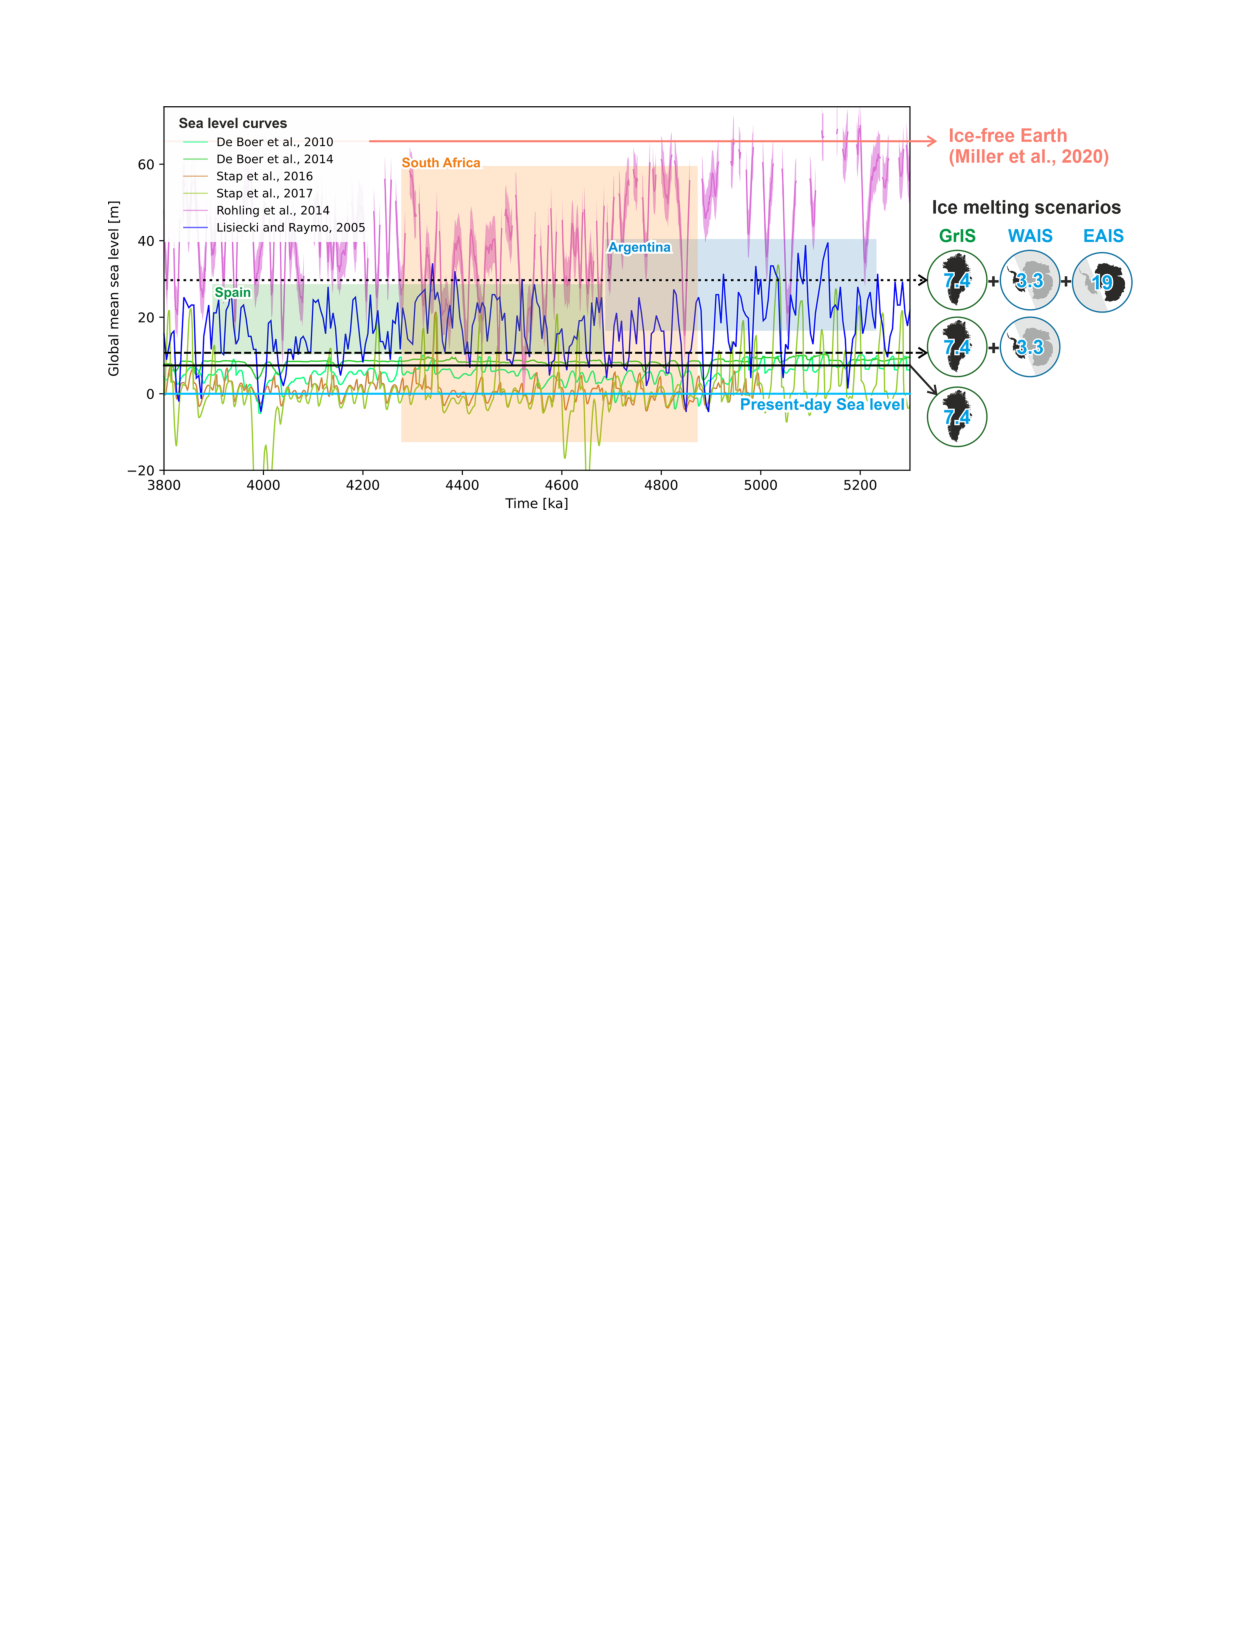
\includegraphics[width=0.9\linewidth]{figures/composite_image.pdf}
    \caption{Esempio di grafico realizzato utilizzando dati da altre pubblicazioni e dati originali, da \cite{rovere_higher_2020}, pubblicato con licenza CC-BY 4.0 - https://creativecommons.org/licenses/by/4.0. La didascalia originale recita: 
    \textit{Comparison between sea-level data discussed in this study and global mean sea level derived from ice models \parencite{deBoer2010,deBoer2014,stap2016,stap2017} and indirect sea level proxies \parencite{rohling2014sea,lisiecki2005pliocene}. The blue curve shows the GMSL prediction that is used in the GIA model and based on scaling the benthic oxygen isotope record by \cite{lisiecki2005pliocene} following the steps described in the methods. Age ranges for observations are 2$\sigma$, while elevation ranges are 1$\sigma$ for Argentina and South Africa, and 16\textsuperscript{th}-84\textsuperscript{th} percentiles for Spain. Horizontal black lines and graphics on the right side of the graph show total sea level equivalent for ice-free Greenland (GrIS, solid line, \cite{morlighem2017bedmachine}), melting of West Antarctic Ice Sheet (WAIS, dashed line \cite{bamber2009reassessment})  and marine sectors of the East Antarctic Ice Sheet (EAIS, dotted line \cite{fretwell2013bedmap2}). The upper red line shows GMSL in an ice-free Earth, estimated to 66m by \cite{Miller1346}.}}
    \label{fig:citations_figure}
\end{figure*}

Nella stesura di documenti diversi da un articolo scientifico, come tesi di laurea o dottorato, o documenti e report tecnici, può essere necessario inserire immagini prese da fonti terze, quindi non prodotte originariamente da uno degli autori del documento. In questo caso, è fondamentale prestare molta attenzione, poiché le immagini utilizzate potrebbero essere soggette a copyright da parte degli autori originali. L’uso non autorizzato di tali immagini può comportare un’infrazione di copyright (\textit{copyright infringement}), che può configurarsi come plagio, reato punibile ai sensi della legge 475/1925, modificata nel 1999. È bene ricordare che il \textit{copyright infringement} non rappresenta solo un reato, ma può anche provocare un danno economico al detentore del copyright. Un esempio classico è quello che ha coinvolto la rock band inglese Queen (insieme a David Bowie) e il rapper americano Vanilla Ice, accusato in sede civile di aver usato nella sua hit “Ice Ice Baby” il giro di basso di “Under Pressure” (composta dai Queen e da Bowie) senza autorizzazione e senza pagare i diritti \parencite{plagioQueen}. La vicenda si è risolta con un pagamento di circa 4 milioni di dollari da parte del rapper ai musicisti inglesi.

Quando si intende usare un’immagine di terzi nel proprio lavoro, la prima cosa da fare è verificare chi sia il detentore del copyright e quale sia la licenza con cui l’immagine è stata pubblicata. Se l’immagine è protetta da copyright, è necessario richiedere il permesso al detentore per poterla utilizzare. In ambito scientifico, è importante ricordare che, per la maggior parte degli articoli scientifici pubblicati da riviste internazionali, il copyright è stato trasferito dall’autore all’editore (ad esempio, Elsevier, Springer, Wiley, ecc.), per cui il permesso va richiesto a quest’ultimo e non all’autore. Molte riviste scientifiche aderiscono alla piattaforma \href{https://www.copyright.com/solutions-rightslink-scientific-communications/}{RightsLink}, che aiuta a individuare chi detiene il copyright di un articolo scientifico e consente, se necessario, di acquistare i diritti su una figura.

Nei paesi anglosassoni, e parzialmente anche in Italia, esiste la possibilità di usare liberamente parti di materiale protetto da copyright secondo la dottrina del \textit{fair use}, che tutela l’utilizzo di un’opera per finalità di critica, ricerca, insegnamento o interesse pubblico. Anche la legge italiana sul Diritto d’Autore (L. 22 aprile 1941, n. 633, e successive modifiche) protegge parzialmente questi usi all’articolo 70, riportato di seguito.

\textbf{L. 22 aprile 1941, n. 633, articolo 70}
\begin{enumerate}
\item \textit{Il riassunto, la citazione o la riproduzione di brani o di parti di opera e la loro comunicazione al pubblico sono liberi se effettuati per uso di critica o di discussione, nei limiti giustificati da tali fini e purché non costituiscano concorrenza all'utilizzazione economica dell'opera; se effettuati a fini di insegnamento o di ricerca scientifica l'utilizzo deve inoltre avvenire per finalità illustrative e per fini non commerciali. \\ 1-bis È consentita la libera pubblicazione attraverso la rete internet, a titolo gratuito, di immagini e musiche a bassa risoluzione o degradate, per uso didattico o scientifico e solo nel caso in cui tale utilizzo non sia a scopo di lucro. Con decreto del Ministro per i beni e le attività culturali, sentiti il Ministro della pubblica istruzione e il Ministro dell'università e della ricerca, previo parere delle Commissioni parlamentari competenti, sono definiti i limiti all'uso didattico o scientifico di cui al presente comma}

\item \textit{ Nelle antologie ad uso scolastico la riproduzione non può superare la misura determinata dal regolamento, il quale fissa la modalità per la determinazione dell'equo compenso.}

\item \textit{ Il riassunto, la citazione o la riproduzione debbono essere sempre accompagnati dalla menzione del titolo dell'opera, dei nomi dell'autore, dell'editore e, se si tratti di traduzione, del traduttore, qualora tali indicazioni figurino sull'opera riprodotta.}
\end{enumerate}

Questo rende possibile, ad esempio, l’uso di immagini in una tesi di dottorato o di laurea. Il \textcite{CRUI} riporta a tal proposito che \textit{”[…] risulta quindi possibile al dottorando utilizzare immagini anche sotto tutela all’interno della tesi che verrà messa online purché la qualità delle immagini sia degradata o a bassa risoluzione”}.

Uno dei principali problemi relativi al cosiddetto \textit{fair use} è che, in caso di controversie, la sua corretta applicazione può essere stabilita solo in sede giudiziaria. In altre parole, non è l’utente dell’immagine a poter determinare se il suo uso ricada tra quelli consentiti dall’Articolo 70, ma, in caso di contestazione, il giudice può stabilire se tutti i requisiti dell’articolo sono stati rispettati e quindi se l’uso dell’immagine sia lecito. Nulla impedisce, comunque, alla persona o all’ente che detiene il copyright di citare in giudizio l’utente che ha usato l'immagine.

La legislazione sul copyright è molto complessa e varia a seconda delle nazioni, quindi non è sempre semplice, durante la stesura di un documento tecnico-scientifico, orientarsi tra le diverse norme o ottenere i necessari permessi dai titolari del copyright. Una regola di base, specialmente per i materiali trovati in rete, è considerare qualsiasi immagine o grafico come proprietà di terzi, e sapere che appropriarsi di tali immagini senza autorizzazione equivale a un furto.

Per evitare questi problemi, la soluzione migliore (oltre alla creazione di immagini originali) è cercare immagini di pubblico dominio o coperte da licenze Creative Commons.

Le immagini di pubblico dominio sono quelle non soggette a copyright, poiché il loro autore ha rinunciato ai diritti o perché il periodo di protezione legale del copyright è scaduto. Le opere create da autori deceduti da oltre 70 anni, o quelle pubblicate da enti governativi (come le immagini della NASA), spesso rientrano nel pubblico dominio. L’uso di immagini di pubblico dominio è completamente libero: possono essere copiate, modificate e distribuite senza la necessità di ottenere permessi o citare l’autore. Tuttavia, è sempre buona pratica riconoscere la fonte originale dell’immagine, anche se non richiesto dalla legge, per garantire trasparenza e correttezza accademica. È anche buona pratica indicare da dove l'immagine é stata scaricata. Per esempio, la famosa immagine \textit{"Blue Marble"} della NASA é di pubblico dominio (\autoref{fig:marble}) e puó essere scaricata da Wikimedia Commons.

\begin{figure}[h!]
    \centering
    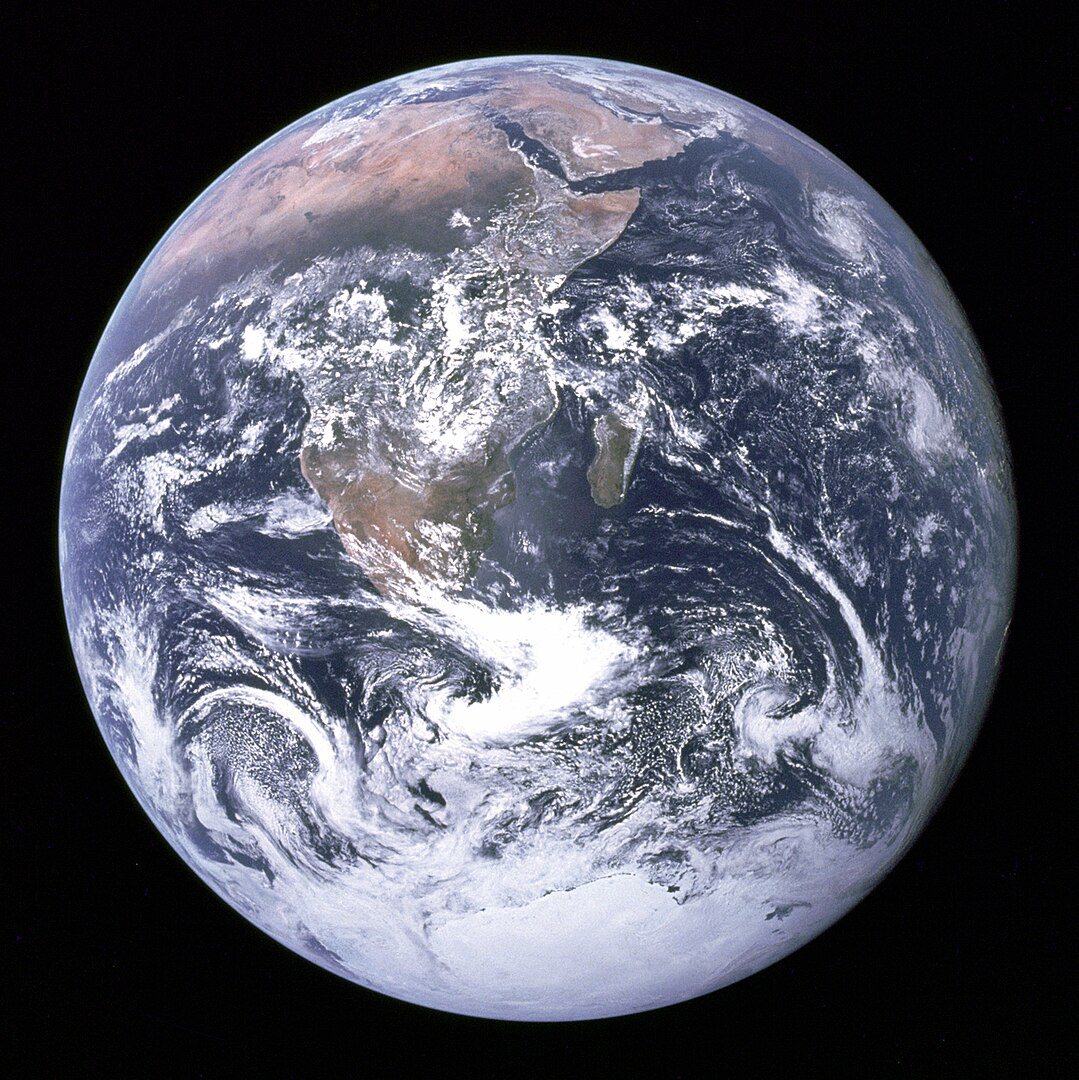
\includegraphics[width=0.8\linewidth]{figures/BlueMarble.jpg}
    \caption{Esempio di immagine di pubblico dominio, la foto del pianeta Terra chiamata "The Blue Marble", scattata dall'equipaggio della NASA/Apollo 17 (Harrison Schmitt o Ron Evans), dominio pubblico (scaricata da \href{(https://en.wikipedia.org/wiki/File:The_Earth_seen_from_Apollo_17.jpg}{Wikimedia Commons} il 27 Settembre 2024).}
    \label{fig:marble}
\end{figure}

Le licenze Creative Commons offrono un modo flessibile per utilizzare immagini prodotte da terzi, permettendo agli autori di concedere alcuni diritti d’uso mantenendo comunque il copyright. Esistono diverse tipologie di licenze Creative Commons, che possono variare dalla più permissiva (“CC0” o “public domain dedication”) a quelle che richiedono l’attribuzione dell’autore (“CC BY”) o limitano l’uso commerciale (“CC BY-NC”). È fondamentale leggere attentamente i termini della licenza per ogni immagine Creative Commons, in quanto alcune possono anche vietare la modifica dell’opera o richiedere che eventuali derivazioni siano distribuite con la stessa licenza dell’originale. L’uso corretto di immagini con licenza Creative Commons richiede sempre l’attribuzione dell’autore originale, specificando chiaramente la licenza con cui l’immagine è stata rilasciata. Per esempio, l'immagine in \autoref{fig:grotta} é stata caricata su Wikimedia Commons con licenza Creative Commons Attribution Share-Alike (\href{https://creativecommons.org/licenses/by-sa/4.0}{CC BY-SA 4.0}, le cui condizioni (tradotte in molte lingue) sono visibili a questa pagina: \url{https://creativecommons.org/licenses/by-sa/4.0/deed.it}. 

\begin{figure}[h!]
    \centering
    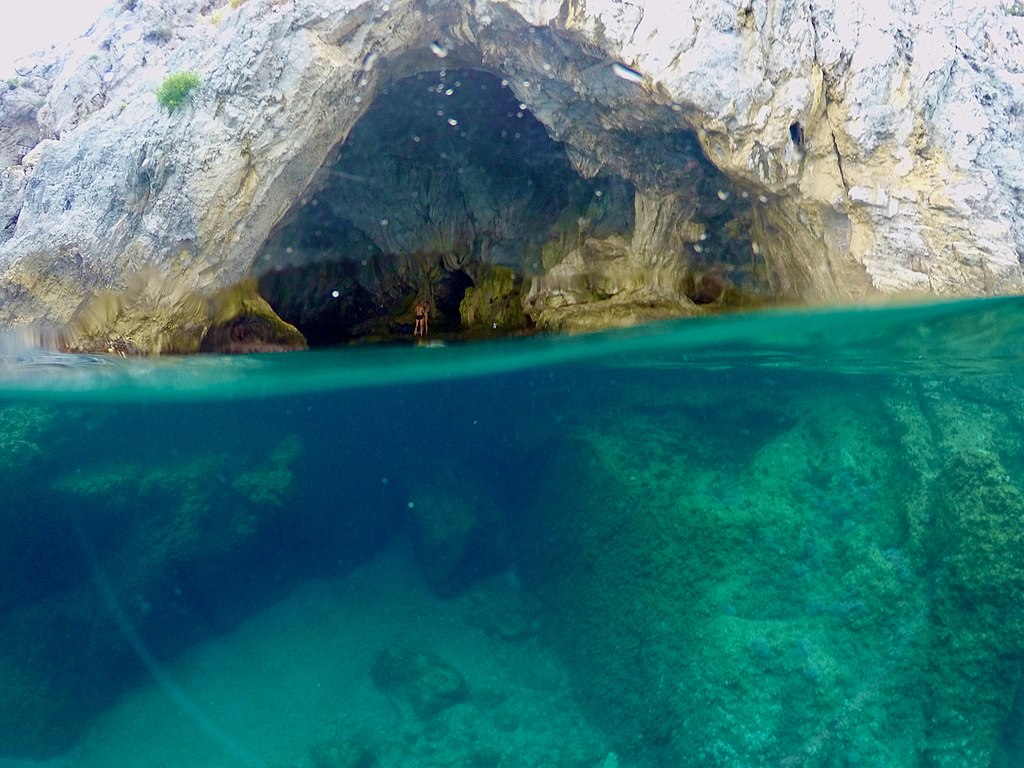
\includegraphics[width=0.8\linewidth]{figures/1024px-Marine_cave_Bergeggi.jpg}
    \caption{Esempio di immagine rilasciata con licenza Creative Commons Attribution Share-Alike (\href{https://creativecommons.org/licenses/by-sa/4.0}{CC BY-SA 4.0}), (Alessio Rovere, scaricata da \href{(https://commons.wikimedia.org/wiki/File:Marine_cave_Bergeggi.jpg}{Wikimedia Commons} il 27 Settembre 2024).}
    \label{fig:grotta}
\end{figure}

Una tabella riassuntiva delle varie licenze Creative Commons è presentata in \autoref{tab:creative_commons}. I dettagli sulle licenze sono disponibili al sito \url{https://creativecommons.org/share-your-work/cclicenses/}.

\begin{table*}[ht!]
\centering
\begin{tabular}{llll}
\hline
\textbf{Licenza Creative Commons} & \textbf{Uso commerciale} & \textbf{Modifiche/Derivazioni} & \textbf{Attribuzione necessaria} \\ \hline
CC BY                             & Consentito               & Consentite                      & Sì                              \\
CC BY-SA                          & Consentito               & Consentite, ma con stessa licenza & Sì                              \\
CC BY-NC                          & Non consentito           & Consentite                      & Sì                              \\ 
CC BY-NC-SA                       & Non consentito           & Consentite, ma con stessa licenza & Sì                              \\
CC BY-ND                          & Consentito               & Non consentite                  & Sì                              \\ 
CC BY-NC-ND                       & Non consentito           & Non consentite                  & Sì                              \\ \hline
\end{tabular}
\caption{Riassunto delle licenze Creative Commons e usi consentiti. Le informazioni dettagliate su ogni licenza sono disponibili al sito \url{https://creativecommons.org/share-your-work/cclicenses/}}
\label{tab:creative_commons}

\end{table*}

\section{Conclusioni}

La redazione di un documento tecnico-scientifico richiede precisione, chiarezza e una solida struttura che guidi il lettore attraverso i vari contenuti. L’uso corretto di figure, tabelle, citazioni e risorse tecniche come i software di scrittura e gestione bibliografica contribuisce a garantire un lavoro di qualità. Inoltre, il rispetto delle norme accademiche, come l’evitare il plagio e l’uso responsabile delle fonti, è essenziale per mantenere l’integrità scientifica del documento. Seguendo queste linee guida e adottando le best practices, è possibile creare un lavoro scientifico professionale e rigoroso.

\section*{Note}
In alcune sezioni di questo documento, è stato utilizzato ChatGPT come supporto per migliorare la struttura e la scorrevolezza di alcuni paragrafi. In particolare, ChatGPT è stato impiegato per ottimizzare il linguaggio, suggerire riformulazioni e migliorare la fluidità dei concetti, come nel caso della rielaborazione del primo paragrafo e nella creazione di esempi. L'autore ha sempre mantenuto il controllo critico sul contenuto e ha citato l’uso di questo strumento, come richiesto nelle pratiche accademiche. ChatGPT è stato un aiuto complementare, ma la supervisione, la validazione dei dati e l’elaborazione scientifica sono rimaste sotto la piena responsabilità dell'autore del testo.

Per quanto riguarda le sezioni relative al plagio e al copyright, questo documento ha scopo puramente informativo e fornisce consigli generali sull’utilizzo di immagini e contenuti da fonti terze. Non costituisce consulenza legale e non può sostituire il parere di un professionista legale qualificato. Per questioni specifiche relative a copyright, licenze e utilizzo di materiale protetto, si consiglia di consultare un avvocato o un esperto legale specializzato in proprietà intellettuale.

\section*{Ringraziamenti}
Desidero ringraziare il Prof. Carlo Nike Bianchi e la Prof.ssa Carla Morri per la revisione critica del testo. Molte delle buone pratiche riportate in questo testo sono frutto dei loro insegnamenti durante la stesura delle mie tesi di laurea e dottorato, e di numerosi articoli scientifici scritti insieme. Ribgrazio la Prof.ssa Barbara Stenni per la rilettura critica del testo.

%----------------------------------------------------------
\printbibliography
%----------------------------------------------------------

\end{document}



